%% template for Sweave vignettes
%\VignetteIndexEntry{HE plot examples}
%\VignetteDepends{candisc,car,lattice,reshape2}
%\VignetteKeywords{MANOVA, ANOVA, Canonical discriminant analysis, effect plots, HE plots}
%\VignettePackage{heplots}

\documentclass[11pt]{article}
\usepackage{float,graphicx,geometry}
\usepackage{amssymb, amsmath, amsfonts}
\usepackage{latexsym}
\usepackage{Sweave}
\usepackage{fancyvrb}
\usepackage{color}
\usepackage{url}
\usepackage[round]{natbib}
\usepackage{hyperref}
\bibliographystyle{abbrvnat}
%\bibpunct{(}{)}{;}{a}{,}{,}
\usepackage{bm}
\usepackage{upquote}
%\usepackage{sfheaders}
\usepackage{xspace}
%\usepackage{multicol}   % for table of contents
\usepackage[toc]{multitoc}   % for table of contents

\geometry{left=1.2in, right=1.2in, top=1in, bottom=1in}

% math stuff
\newcommand*{\given}{\ensuremath{\, | \,}}
\renewcommand*{\vec}[1]{\ensuremath{\bm{#1}}}
\newcommand{\mat}[1]{\ensuremath{\bm{#1}}}
\newcommand{\trans}{\ensuremath{^\mathsf{T}}}
\newcommand{\diag}[1]{\ensuremath{\mathrm{diag} (#1)}}
%\def\binom#1#2{{#1 \choose #2}}%
%\newcommand{\implies}{ \ensuremath{\mapsto} }

\newcommand{\sizedmat}[2]{%
  \mathord{\mathop{\mat{#1}}\limits_{(#2)}}%
}


\newcommand*{\LM}{LM}
\newcommand*{\MLM}{MvLM\xspace}
\newcommand*{\MLMs}{MvLMs\xspace}
\newcommand*{\Var}{\ensuremath{\mathsf{Var}}}


%\newenvironment{equation*}{\displaymath}{\enddisplaymath}%

\newcommand{\tabref}[1]{Table~\ref{#1}}
\newcommand{\figref}[1]{Figure~\ref{#1}}
\newcommand{\secref}[1]{Section~\ref{#1}}
\newcommand{\loglin}{loglinear }

% R stuff
\newcommand{\pkg}[1]{{\textsf{#1} package}}
\newcommand{\Rpackage}[1]{{\textsf{#1}}}
\newcommand{\R}{\textsf{R}\xspace}
\newcommand{\code}[1]{{\texttt{#1}}}
\newcommand{\func}[1]{{\texttt{#1()}}}


\title{HE Plot Examples}
\author{Michael Friendly}
\date{\footnotesize{Using \Rpackage{heplots} version 1.0-2
	and \Rpackage{candisc} version 0.5-23; Date: 2012-12-13}}


\definecolor{Soutput}{rgb}{0,0,0.56}
\definecolor{Sinput}{rgb}{0.56,0,0}
\DefineVerbatimEnvironment{Sinput}{Verbatim}{formatcom={\color{Sinput}},fontsize=\footnotesize, baselinestretch=0.75}
\DefineVerbatimEnvironment{Soutput}{Verbatim}{formatcom={\color{Soutput}},fontsize=\footnotesize, baselinestretch=0.75}


\begin{document}
\maketitle

\begin{minipage}[b]{.3\linewidth}
	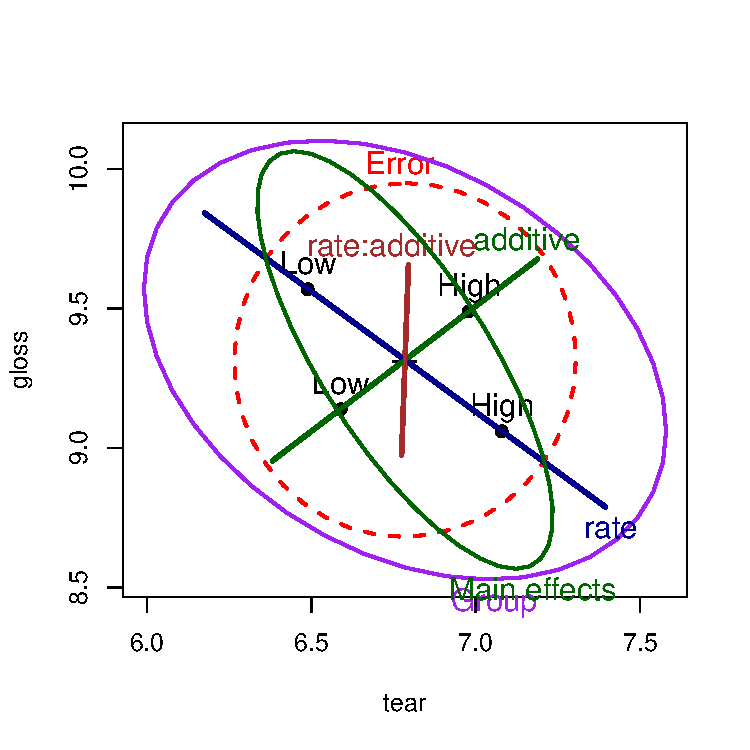
\includegraphics[width=\linewidth, trim=0 30 0 30]{fig/plot-plastic2}
\end{minipage}
\begin{minipage}[b]{.3\linewidth}
	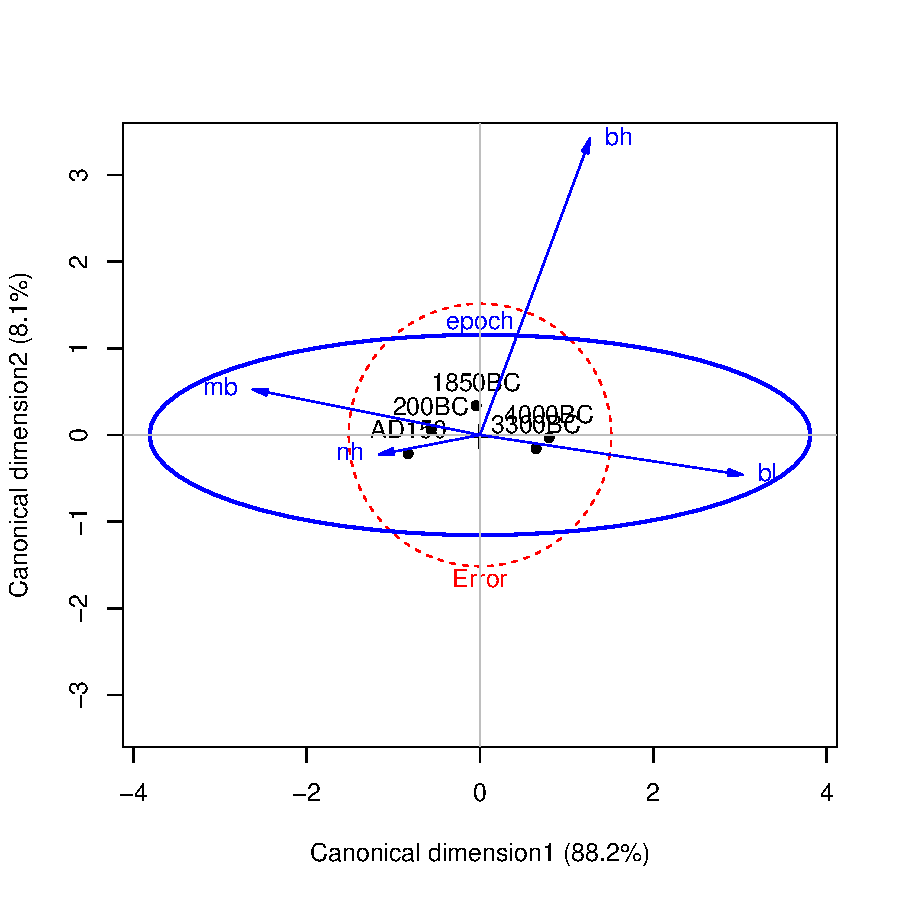
\includegraphics[width=\linewidth, trim=0 30 0 30]{fig/plot-skulls-can2}
\end{minipage}
\begin{minipage}[b]{.3\linewidth}
	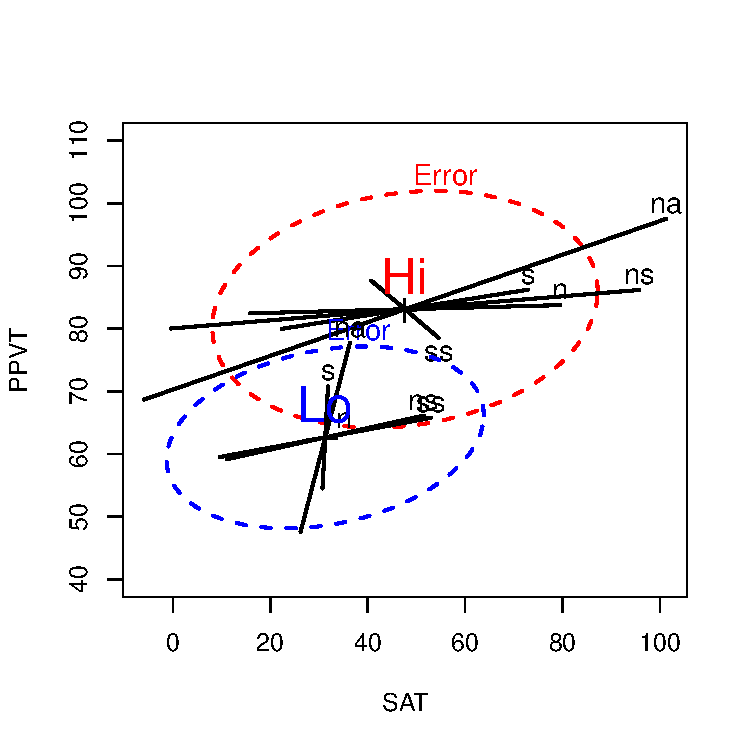
\includegraphics[width=\linewidth, trim=0 30 0 30]{fig/plot-rohwer-HE1}
\end{minipage}


\begin{abstract}
	This vignette provides some worked examples of the analysis of multivariate linear models 
	(\MLMs)
	with graphical methods for visualizing results using the \pkg{heplots} and the \pkg{candisc}.
	The emphasis here is on using these methods in \R, and understanding how they help reveal
	aspects of these models that might not be apparent from other graphical displays.

	No attempt is made here to describe the theory of \MLMs or the statistical details behind
	HE plots and their reduced-rank canonical cousins.
	For that, see \citet{FoxFriendlyMonette:09:compstat,Friendly:07:manova,Friendly:06:hesoft}.
\end{abstract}

{\small
% \sloppy
% \begin{multicols}{2}
 \tableofcontents
% \end{multicols}
}




%\SweaveOpts{concordance=TRUE}
\setkeys{Gin}{width=0.7\textwidth}


\section{MANOVA Designs}

\subsection{Plastic film data}
An experiment was conducted to determine the optimum conditions for extruding plastic film. 
Three responses, \code{tear} resistance, film \code{gloss} and film \code{opacity}
were measured in relation to two factors, \code{rate} of extrusion and amount of an \code{additive},
both of these being set to two values, High and Low.
The design is thus a $2\times 2$ MANOVA, with $n=5$ per cell. 
This example illustrates 2D and 3D HE plots, the difference between 
``effect'' scaling and ``evidence'' (significance) scaling, and visualizing
composite linear hypotheses.

We begin with an overall MANOVA for the two-way MANOVA model.
Because each effect has 1 df, all of the multivariate statistics are equivalent,
but we specify \code{test.statistic="Roy"} because Roy's test has
a natural visual interpretation in HE plots.
\begin{Schunk}
\begin{Sinput}
> plastic.mod <- lm(cbind(tear, gloss, opacity) ~ rate*additive, data=Plastic)
> Anova(plastic.mod, test.statistic="Roy")
\end{Sinput}
\begin{Soutput}
Type II MANOVA Tests: Roy test statistic
              Df test stat approx F num Df den Df Pr(>F)   
rate           1     1.619     7.55      3     14  0.003 **
additive       1     0.912     4.26      3     14  0.025 * 
rate:additive  1     0.287     1.34      3     14  0.302   
---
Signif. codes:  0 '***' 0.001 '**' 0.01 '*' 0.05 '.' 0.1 ' ' 1 
\end{Soutput}
\end{Schunk}
For the three responses jointly, the main effects of  \code{rate} and \code{additive}
are significant, while their interaction is not.
In some approaches to testing effects in multivariate linear models (\MLM),
significant multivariate tests are often followed by univariate tests on each
of the responses separately to determine which responses contribute to each
significant effect.  In \R, these analyses are most convieniently performed
using the \func{update} method for the \code{mlm} object \code{plastic.mod}.
\begin{Schunk}
\begin{Sinput}
> Anova(update(plastic.mod, tear ~ .))
\end{Sinput}
\begin{Soutput}
Anova Table (Type II tests)

Response: tear
              Sum Sq Df F value Pr(>F)   
rate            1.74  1    15.8 0.0011 **
additive        0.76  1     6.9 0.0183 * 
rate:additive   0.00  1     0.0 0.9471   
Residuals       1.76 16                  
---
Signif. codes:  0 '***' 0.001 '**' 0.01 '*' 0.05 '.' 0.1 ' ' 1 
\end{Soutput}
\begin{Sinput}
> Anova(update(plastic.mod, gloss ~ .))
\end{Sinput}
\begin{Soutput}
Anova Table (Type II tests)

Response: gloss
              Sum Sq Df F value Pr(>F)  
rate           1.300  1    7.92  0.012 *
additive       0.612  1    3.73  0.071 .
rate:additive  0.544  1    3.32  0.087 .
Residuals      2.628 16                 
---
Signif. codes:  0 '***' 0.001 '**' 0.01 '*' 0.05 '.' 0.1 ' ' 1 
\end{Soutput}
\begin{Sinput}
> Anova(update(plastic.mod, opacity ~ .))
\end{Sinput}
\begin{Soutput}
Anova Table (Type II tests)

Response: opacity
              Sum Sq Df F value Pr(>F)
rate             0.4  1    0.10   0.75
additive         4.9  1    1.21   0.29
rate:additive    4.0  1    0.98   0.34
Residuals       64.9 16               
\end{Soutput}
\end{Schunk}
The results above show significant main effects for \code{tear},
a significant main effect of \code{rate} for \code{gloss},
and no significant effects for \code{opacity}, but they don't shed light on the
\emph{nature} of these effects.
Traditional univariate plots of the means for each variable separately
are useful, but they don't allow visualization of the
\emph{relations} among the response variables.

We can visualize these
effects for pairs of variables in an HE plot, showing the ``size'' and
orientation of hypothesis variation (\mat{H}) in relation to error
variation (\mat{E}) as ellipsoids.
When, as here, the model terms have 1 degree of freedom, the
\mat{H} ellipsoids degenerate to a line.
\begin{Schunk}
\begin{Sinput}
> # Compare evidence and effect scaling 
> colors = c("red", "darkblue", "darkgreen", "brown")
> heplot(plastic.mod, size="evidence", col=colors, cex=1.25)
> heplot(plastic.mod, size="effect", add=TRUE, lwd=4, term.labels=FALSE, col=colors)
\end{Sinput}
\end{Schunk}
With effect scaling, both the \mat{H} and \mat{E} sums of squares and products
matrices are both divided by the error df, giving multivariate analogs of univariate
measures of effect size, e.g., $(\bar{y}_1-\bar{y}_2) / s$.
With significance scaling, the \mat{H} ellipse is further divided by
$\lambda_\alpha$, the critical value of Roy's largest root statistic.
This scaling has the property that an \mat{H} ellipse will protrude somewhere
outside the \mat{E} ellipse \emph{iff} the
multivariate test is significant at level $\alpha$.
\figref{fig:plastic1} shows both scalings, using a thinner line for significance scaling.
Note that the (degenerate) ellipse for \code{additive} is significant, but
does not protrude outside the \mat{E} ellipse in this view.
All that is guarranteed is that it will protrude somewhere in the 3D space of
the responses.


By design, means for the levels of interaction terms are not shown in the HE plot,
because doing so in general can lead to messy displays.
We can add them here for the term \code{rate:additive} as follows:
\begin{Schunk}
\begin{Sinput}
> ## add interaction means
> intMeans <- termMeans(plastic.mod, 'rate:additive', abbrev.levels=2)
> #rownames(intMeans) <- apply(expand.grid(c('Lo','Hi'), c('Lo', 'Hi')), 1, paste, collapse=':')
> points(intMeans[,1], intMeans[,2], pch=18, cex=1.2, col="brown")
> text(intMeans[,1], intMeans[,2], rownames(intMeans), adj=c(0.5,1), col="brown")
> lines(intMeans[c(1,3),1], intMeans[c(1,3),2], col="brown")
> lines(intMeans[c(2,4),1], intMeans[c(2,4),2], col="brown")
\end{Sinput}
\end{Schunk}

\begin{figure}[htb]
\begin{center}
	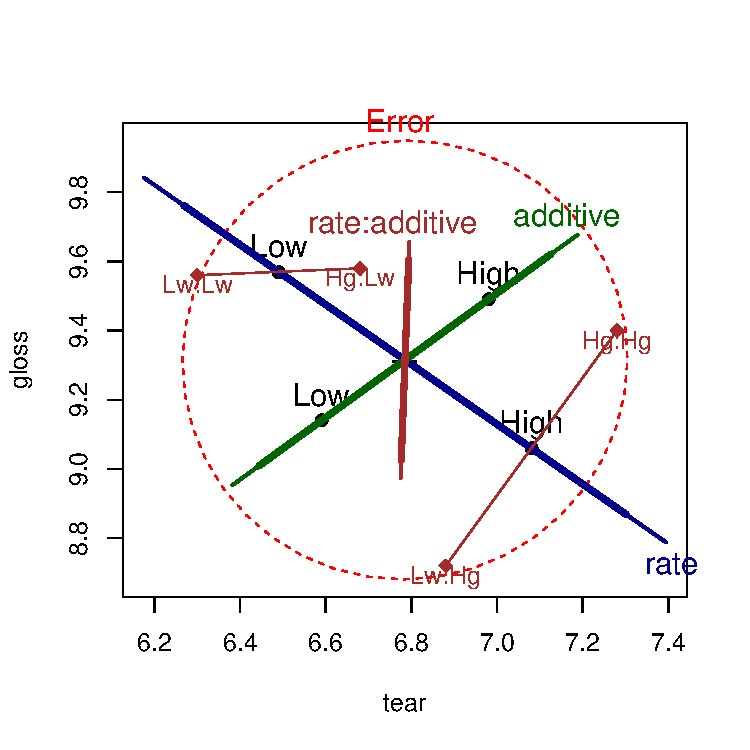
\includegraphics[width=.6\textwidth, clip]{plot-plastic1}
\caption{HE plot for effects on \code{tear} and \code{gloss} according to the
	factors \code{rate}, \code{additive} and their interaction, \code{rate:additive}.
	 The thicker
	lines show effect size scaling, the thinner lines show significance scaling.}
\label{fig:plastic1}
\end{center}
\end{figure}


The factor means in this plot (\figref{fig:plastic1}) have a simple interpretation:
The high \code{rate} level yields greater \code{tear} resistance but lower \code{gloss}
than the low level.
The high \code{additive} amount produces greater \code{tear} resistance and greater \code{gloss}.

The \code{rate:additive} interaction is not significant overall, though it
approaches significance for \code{gloss}. 
The cell means for the combinations
of \code{rate} and \code{additive} shown in this figure suggest an explanation,
for tutorial purposes:
with the low level of \code{rate}, there is little difference in \code{gloss}
for the levels of \code{additive}. At the high level of \code{rate}, there is
a larger difference in \code{gloss}.  The \mat{H} ellipse for the interaction
of \code{rate:additive} therefore ``points'' in the direction of \code{gloss}
indicating that this variable contributes to the interaction in the 
multivariate tests.


In some MANOVA models, it is of interest to test sub-hypotheses 
of a given main effect or interaction, or conversely to test composite
hypotheses that pool together certain effects to test them jointly.
All of these tests (and, indeed, the tests of terms in a given model)
are carried out as tests of general linear hypotheses in the \MLM.

In this example, it might be useful to test two composite hypotheses:
one corresponding to both main effects jointly, and another corresponding
to no difference among the means of the four groups (equivalent to
a joint test for the overall model). These tests are specified in terms
of subsets or linear combinations of the model parameters.
\begin{Schunk}
\begin{Sinput}
> plastic.mod
\end{Sinput}
\begin{Soutput}
Call:
lm(formula = cbind(tear, gloss, opacity) ~ rate * additive, data = Plastic)

Coefficients:
                       tear   gloss  opacity
(Intercept)             6.30   9.56   3.74  
rateHigh                0.58  -0.84  -0.60  
additiveHigh            0.38   0.02   0.10  
rateHigh:additiveHigh   0.02   0.66   1.78  
\end{Soutput}
\end{Schunk}
Thus, for example, the joint test of both main effects tests the parameters
\code{rateHigh} and \code{additiveHigh}.
\begin{Schunk}
\begin{Sinput}
> print(linearHypothesis(plastic.mod, c("rateHigh", "additiveHigh"), title="Main effects"), SSP=FALSE)
\end{Sinput}
\begin{Soutput}
Multivariate Tests: Main effects
                 Df test stat approx F num Df den Df   Pr(>F)   
Pillai            2   0.71161   2.7616      6     30 0.029394 * 
Wilks             2   0.37410   2.9632      6     28 0.022839 * 
Hotelling-Lawley  2   1.44400   3.1287      6     26 0.019176 * 
Roy               2   1.26253   6.3127      3     15 0.005542 **
---
Signif. codes:  0 '***' 0.001 '**' 0.01 '*' 0.05 '.' 0.1 ' ' 1 
\end{Soutput}
\begin{Sinput}
> print(linearHypothesis(plastic.mod, c("rateHigh", "additiveHigh", "rateHigh:additiveHigh"), title="Groups"), SSP=FALSE)
\end{Sinput}
\begin{Soutput}
Multivariate Tests: Groups
                 Df test stat approx F num Df den Df   Pr(>F)    
Pillai            3   1.14560   3.2948      9 48.000 0.003350 ** 
Wilks             3   0.17802   3.9252      9 34.223 0.001663 ** 
Hotelling-Lawley  3   2.81752   3.9654      9 38.000 0.001245 ** 
Roy               3   1.86960   9.9712      3 16.000 0.000603 ***
---
Signif. codes:  0 '***' 0.001 '**' 0.01 '*' 0.05 '.' 0.1 ' ' 1 
\end{Soutput}
\end{Schunk}

Correspondingly, we can display these tests in the HE plot by specifying these tests in the
\code{hypothesis} argument to \func{heplot}, as shown in \figref{fig:plastic2}.
\begin{figure}[htb]
\begin{center}
\begin{Schunk}
\begin{Sinput}
> heplot(plastic.mod, hypotheses=list("Group" = 
         c("rateHigh", "additiveHigh", "rateHigh:additiveHigh ")),
         col=c(colors, "purple"),
         lwd=c(2, 3, 3, 3, 2), cex=1.25)
> heplot(plastic.mod, hypotheses=list("Main effects" = 
         c("rateHigh", "additiveHigh")), add=TRUE,
         col=c(colors, "darkgreen"), cex=1.25)
\end{Sinput}
\end{Schunk}
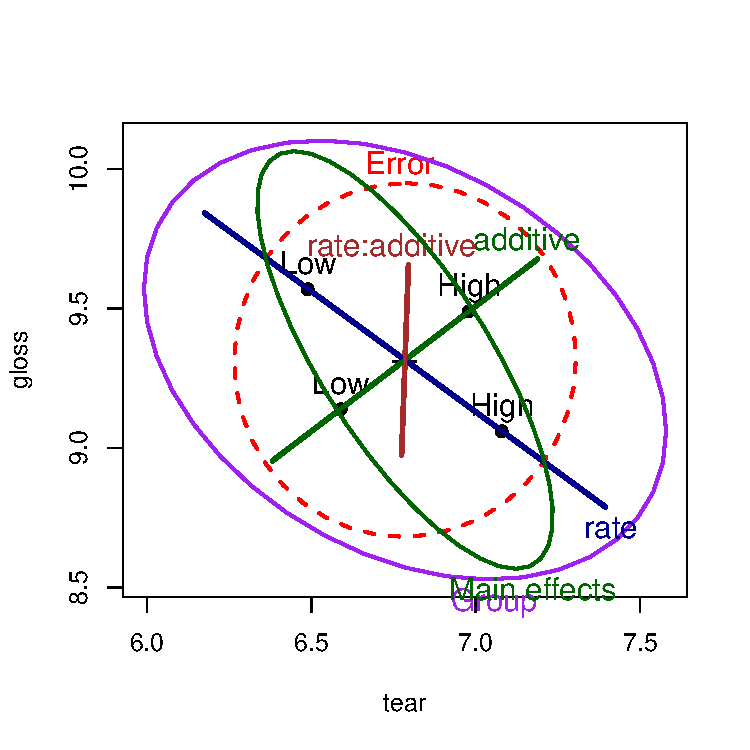
\includegraphics{fig/plot-plastic2}
\caption{HE plot for \code{tear} and \code{gloss}, supplemented with ellipses representing
	the joint tests of main effects and all group differences}
\label{fig:plastic2}
\end{center}
\end{figure}

Finally, a 3D HE plot can be produced with \func{heplot3d}, giving \figref{fig:plastic1-HE3D}.
This plot was rotated interactively to a view that shows both main effects
protruding outside the error ellipsoid.
\begin{Schunk}
\begin{Sinput}
> colors = c("pink", "darkblue", "darkgreen", "brown")
> heplot3d(plastic.mod, col=colors)
\end{Sinput}
\end{Schunk}

\begin{figure}[htb]
\begin{center}
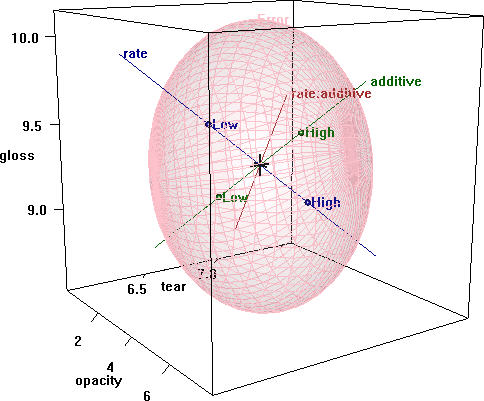
\includegraphics[clip]{plastic1-HE3D}
\caption{3D HE plot for the plastic film data}
\label{fig:plastic1-HE3D}
\end{center}
\end{figure}


\subsection[Mock jury decisions]{Effects of physical attractiveness on mock jury decisions}

In a social psychology
study of influences on jury decisions
by \citet{Plaster:89},
male participants (prison inmates)
were shown a picture of one of three young women.  
Pilot  work
had indicated  that one woman  was beautiful,  another of  average physical
attractiveness, and the third  unattractive.  Participants rated the  woman they
saw on each  of twelve attributes on scales of 1--9.  These measures were used to check on the
manipulation of ``attractiveness'' by the photo.

Then the participants were told that the person in the photo had committed a
Crime, and asked to rate the seriousness of the crime and recommend a
prison sentence, in Years.  The data are contained in the data frame \code{MockJury}.%
\footnote{The data were made available courtesy of Karl Wuensch, from
	\url{http://core.ecu.edu/psyc/wuenschk/StatData/PLASTER.dat}
}

\begin{Schunk}
\begin{Sinput}
> str(MockJury)
\end{Sinput}
\begin{Soutput}
'data.frame':	114 obs. of  17 variables:
 $ Attr         : Factor w/ 3 levels "Beautiful","Average",..: 1 1 1 1 1 1 1 1 1 1 ...
 $ Crime        : Factor w/ 2 levels "Burglary","Swindle": 1 1 1 1 1 1 1 1 1 1 ...
 $ Years        : int  10 3 5 1 7 7 3 7 2 3 ...
 $ Serious      : int  8 8 5 3 9 9 4 4 5 2 ...
 $ exciting     : int  6 9 3 3 1 1 5 4 4 6 ...
 $ calm         : int  9 5 4 6 1 5 6 9 8 8 ...
 $ independent  : int  9 9 6 9 5 7 7 2 8 7 ...
 $ sincere      : int  8 3 3 8 1 5 6 9 7 5 ...
 $ warm         : int  5 5 6 8 8 8 7 6 1 7 ...
 $ phyattr      : int  9 9 7 9 8 8 8 5 9 8 ...
 $ sociable     : int  9 9 4 9 9 9 7 2 1 9 ...
 $ kind         : int  9 4 2 9 4 5 5 9 5 7 ...
 $ intelligent  : int  6 9 4 9 7 8 7 9 9 9 ...
 $ strong       : int  9 5 5 9 9 9 5 2 7 5 ...
 $ sophisticated: int  9 5 4 9 9 9 6 2 7 6 ...
 $ happy        : int  5 5 5 9 8 9 5 2 6 8 ...
 $ ownPA        : int  9 7 5 9 7 9 6 5 3 6 ...
\end{Soutput}
\end{Schunk}
Sample sizes were roughly balanced  for the independent variables
in the three conditions of the attractiveness of the photo,
and the combinations of this with \code{Crime}:
\begin{Schunk}
\begin{Sinput}
> table(MockJury$Attr)
\end{Sinput}
\begin{Soutput}
   Beautiful      Average Unattractive 
          39           38           37 
\end{Soutput}
\begin{Sinput}
> table(MockJury$Attr, MockJury$Crime)
\end{Sinput}
\begin{Soutput}
               Burglary Swindle
  Beautiful          21      18
  Average            18      20
  Unattractive       20      17
\end{Soutput}
\end{Schunk}

The main questions of interest were:
(a) Does attractiveness of the ``defendent'' influence the sentence or perceived
seriousness of the crime?  
(b) Does attractiveness interact with the nature of the
crime?

But first, we try to assess the ratings of the photos in relation to the 
presumed categories of the independent variable \code{Attr}.  The questions here
are (a) do the ratings of the photos on physical attractiveness
(\code{phyattr}) confirm the original classification?
(b) how do other ratings differentiate the photos?
To keep things simple, we consider ony a few of the other ratings in a one-way MANOVA.

\begin{Schunk}
\begin{Sinput}
> (jury.mod1 <- lm( cbind(phyattr, happy, independent, sophisticated) ~ Attr, data=MockJury))
\end{Sinput}
\begin{Soutput}
Call:
lm(formula = cbind(phyattr, happy, independent, sophisticated) ~ 
    Attr, data = MockJury)

Coefficients:
                  phyattr  happy   independent  sophisticated
(Intercept)        8.282    5.359   6.410        6.077       
AttrAverage       -4.808    0.430   0.537       -1.340       
AttrUnattractive  -5.390   -1.359  -1.410       -1.753       
\end{Soutput}
\begin{Sinput}
> Anova(jury.mod1, test="Roy")
\end{Sinput}
\begin{Soutput}
Type II MANOVA Tests: Roy test statistic
     Df test stat approx F num Df den Df Pr(>F)    
Attr  2      1.77     48.2      4    109 <2e-16 ***
---
Signif. codes:  0 '***' 0.001 '**' 0.01 '*' 0.05 '.' 0.1 ' ' 1 
\end{Soutput}
\end{Schunk}
Note that Beautiful is the baseline category of \code{Attr}, so the
intercept term gives the means for this level.
We see that the means are significantly different on all four variables
collectively, by a joint multivariate test.  A traditional analysis might
follow up with univariate ANOVAs for each measure separately. 

As an aid to interpretation of the MANOVA results
We can examine the test of \code{Attr} in this model with an HE plot for
pairs of variables, e.g., for \code{phyattr} and  \code{happy} (\figref{fig:jury-mod1-HE}).
The means in this plot show that Beautiful is rated higher on
physical attractiveness than the other two photos, while Unattractive
is rated less happy than the other two. Comparing the sizes of the
ellipses, differences among group means on physical attractiveness
contributes more to significance than do ratings on happy.

\begin{Schunk}
\begin{Sinput}
> heplot(jury.mod1, main="HE plot for manipulation check")
\end{Sinput}
\end{Schunk}

\begin{figure}[htb]
\begin{center}
	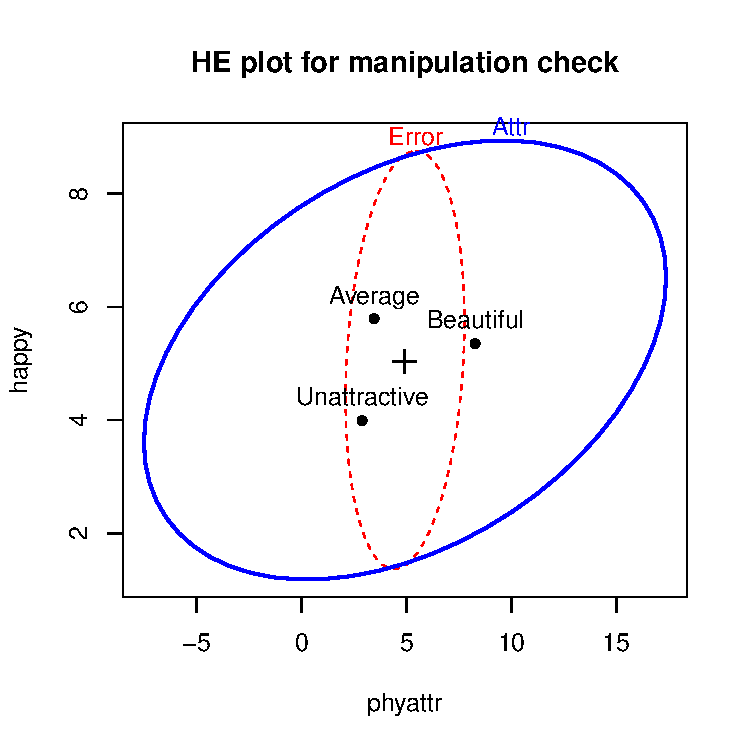
\includegraphics{fig/plot-jury-mod1-HE}
\caption{HE plot for ratings of \code{phyattr} and \code{happy} according to the
	classification of photos on \code{Attr}}
\label{fig:jury-mod1-HE}
\end{center}
\end{figure}

The HE plot for all pairs of variables (\figref{fig:jury-mod1-pairs}) shows that the means for \code{happy}
and \code{independent} are highly correlated, as are the means for \code{phyattr}
and \code{sophisticated}.  In most of these pairwise plots, the means form a
triangle rather than a line, suggesting that these attributes are indeed
measuring different aspects of the photos.

\begin{figure}[htb]
\begin{center}
\begin{Schunk}
\begin{Sinput}
> pairs(jury.mod1)
\end{Sinput}
\end{Schunk}
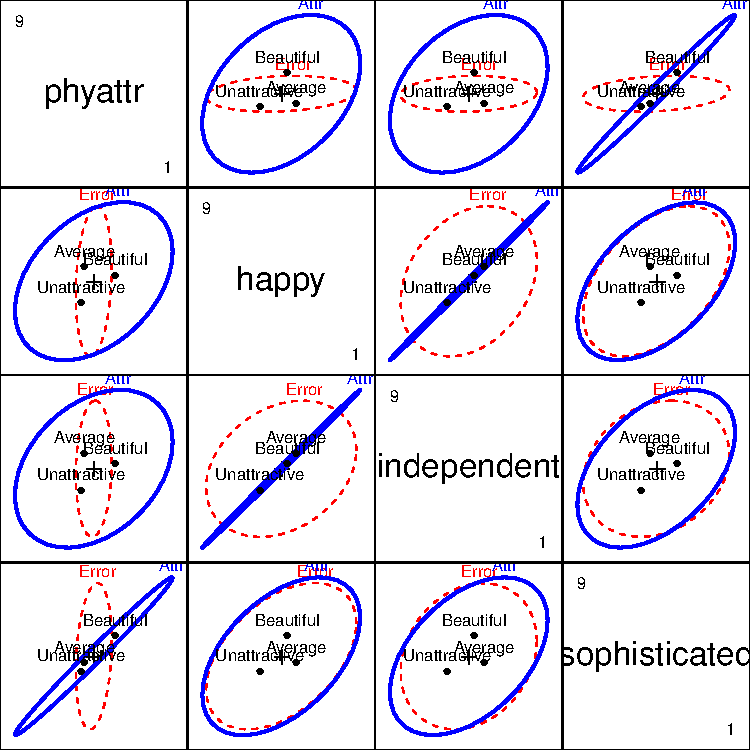
\includegraphics{fig/plot-jury-mod1-pairs}
\caption{HE plots for all pairs of ratings according to the
	classification of photos on \code{Attr}}
\label{fig:jury-mod1-pairs}
\end{center}
\end{figure}

With 3 groups and 4 variables, the \mat{H} ellipsoid has only $s=\min(df_h, p)=2$
dimensions.  \func{candisc} carries out a canonical discriminant analysis
for the \MLM\  and returns an object that can be used to show an HE plot in the
space of the canonical dimensions.  This is plotted in \figref{fig:jury-can1}.

\begin{Schunk}
\begin{Sinput}
> jury.can <- candisc(jury.mod1)
> jury.can
\end{Sinput}
\begin{Soutput}
Canonical Discriminant Analysis for Attr:

  CanRsq Eigenvalue Difference Percent Cumulative
1  0.639      1.767        1.6   91.33       91.3
2  0.144      0.168        1.6    8.67      100.0

Test of H0: The canonical correlations in the 
current row and all that follow are zero

  LR test stat approx F num Df den Df Pr(> F)    
1        0.309     43.9      4    220 < 2e-16 ***
2        0.856     18.6      1    111 3.5e-05 ***
---
Signif. codes:  0 '***' 0.001 '**' 0.01 '*' 0.05 '.' 0.1 ' ' 1 
\end{Soutput}
\end{Schunk}

\begin{figure}[htb]
\begin{center}
\begin{Schunk}
\begin{Sinput}
> opar <- par(xpd=TRUE)
> heplot(jury.can, prefix="Canonical dimension", main="Canonical HE plot")
> par(opar)
\end{Sinput}
\end{Schunk}
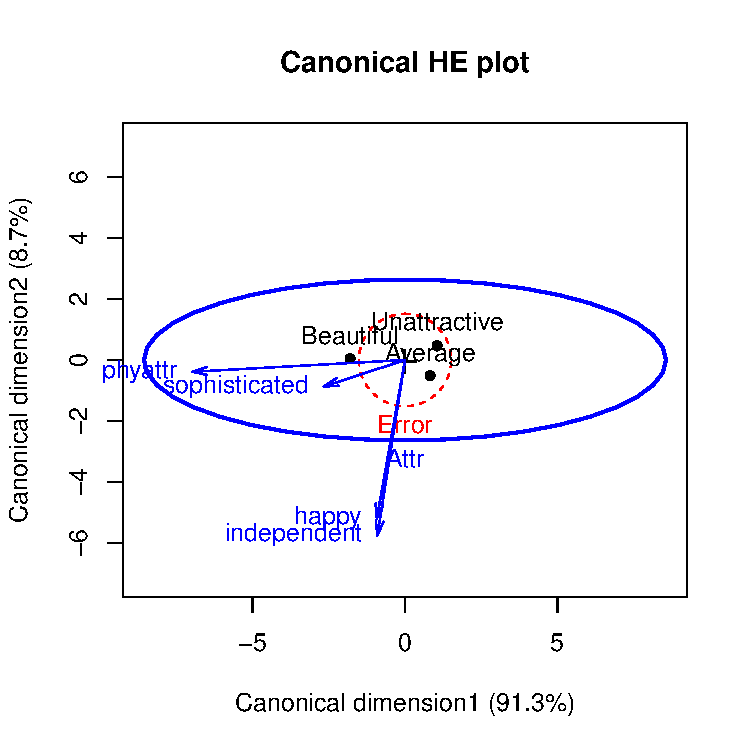
\includegraphics{fig/plot-jury-can1}
\caption{Canonical discriminant HE plot for the MockJury data}
\label{fig:jury-can1}
\end{center}
\end{figure}

From this we can see that 91\% of the variation among group means
is accounted for by the first dimension, and this is nearly completely
aligned with \code{phyattr}. 
The second dimension, accounting for the remaining 9\%
is determined nearly entirely by ratings on \code{happy} and \code{independent}.
This display gives a relatively simple account of the results of the MANOVA
and the relations of each of the ratings to discrimination among the photos.

Proceeding to the main questions of interest, we carry out a two-way MANOVA of the responses
\code{Years} and \code{Serious} in relation to the independent variables
\code{Attr} and \code{Crime}.

\begin{Schunk}
\begin{Sinput}
> # influence of Attr of photo and nature of crime on Serious and Years
> jury.mod2 <- lm( cbind(Serious, Years) ~ Attr * Crime, data=MockJury)
> Anova(jury.mod2, test="Roy")
\end{Sinput}
\begin{Soutput}
Type II MANOVA Tests: Roy test statistic
           Df test stat approx F num Df den Df Pr(>F)  
Attr        2    0.0756     4.08      2    108  0.020 *
Crime       1    0.0047     0.25      2    107  0.778  
Attr:Crime  2    0.0501     2.71      2    108  0.071 .
---
Signif. codes:  0 '***' 0.001 '**' 0.01 '*' 0.05 '.' 0.1 ' ' 1 
\end{Soutput}
\end{Schunk}
We see that there is a nearly significant  interaction between \code{Attr} and \code{Crime}
and a strong effect of \code{Attr}.

\begin{figure}[htb]
\begin{center}
\begin{Schunk}
\begin{Sinput}
> heplot(jury.mod2)
\end{Sinput}
\end{Schunk}
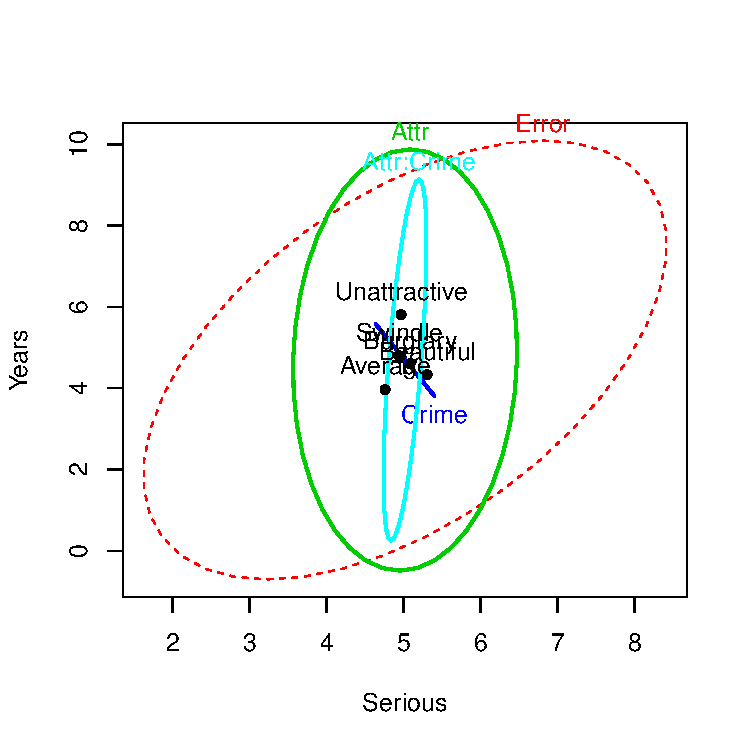
\includegraphics{fig/plot-jury-mod2-HE}
\caption{HE plot for the two-way MANOVA for \code{Years} and \code{Serious}}
\label{fig:jury-mod2-HE}
\end{center}
\end{figure}

The HE plot shows that the nearly significant
interaction of \code{Attr:Crime} is mainly in terms of
differences among the groups on the response of \code{Years} of sentence,
with very little contribution of \code{Serious}.  We explore this interaction in a bit more detail
below.  The main effect of \code{Attr} is also dominated by differences among groups
on \code{Years}. 

If we assume that \code{Years} of sentence is the main outcome of interest,
it also makes sense to carry out a step-down test of this variable by itself,
controlling for the rating of seriousness (\code{Serious}) of the crime.
The model \code{jury.mod3} below is equivalent to an ANCOVA for \code{Years}.
\begin{Schunk}
\begin{Sinput}
> # stepdown test (ANCOVA), controlling for Serious
> jury.mod3 <- lm( Years ~ Serious + Attr * Crime, data=MockJury)
> t(coef(jury.mod3))
\end{Sinput}
\begin{Soutput}
     (Intercept) Serious AttrAverage AttrUnattractive CrimeSwindle
[1,]    0.011612 0.83711     0.39586          0.60285     -0.26302
     AttrAverage:CrimeSwindle AttrUnattractive:CrimeSwindle
[1,]                 -0.53701                        2.5123
\end{Soutput}
\begin{Sinput}
> Anova(jury.mod3)
\end{Sinput}
\begin{Soutput}
Anova Table (Type II tests)

Response: Years
           Sum Sq  Df F value  Pr(>F)    
Serious       379   1   41.14 3.9e-09 ***
Attr           74   2    4.02   0.021 *  
Crime           4   1    0.43   0.516    
Attr:Crime     49   2    2.67   0.074 .  
Residuals     987 107                    
---
Signif. codes:  0 '***' 0.001 '**' 0.01 '*' 0.05 '.' 0.1 ' ' 1 
\end{Soutput}
\end{Schunk}
Thus, even when adjusting for \code{Serious} rating, there is still a 
significant main effect of \code{Attr} of the photo, but also a hint of
an interaction of \code{Attr} with \code{Crime}. The coefficient for
\code{Serious} indicates that participants awarded 0.84 additional
years of sentence for each 1 unit step on the scale of seriousness of crime.

A particularly useful
method for visualizing the fitted effects in such univariate response
models is provided by the \pkg{effects}.  By default \func{allEffects}
calculates the predicted values for all high-order terms in a given
model, and the \code{plot} method produces plots of these values for
each term.  The statements below produce \figref{fig:jury-mod3-eff}.

\setkeys{Gin}{width=1\textwidth}
\begin{Schunk}
\begin{Sinput}
> library(effects)
> jury.eff <- allEffects(jury.mod3)
> plot(jury.eff, ask=FALSE)
\end{Sinput}
\end{Schunk}

\begin{figure}[htb!] % maybe use [H]
\begin{center}
	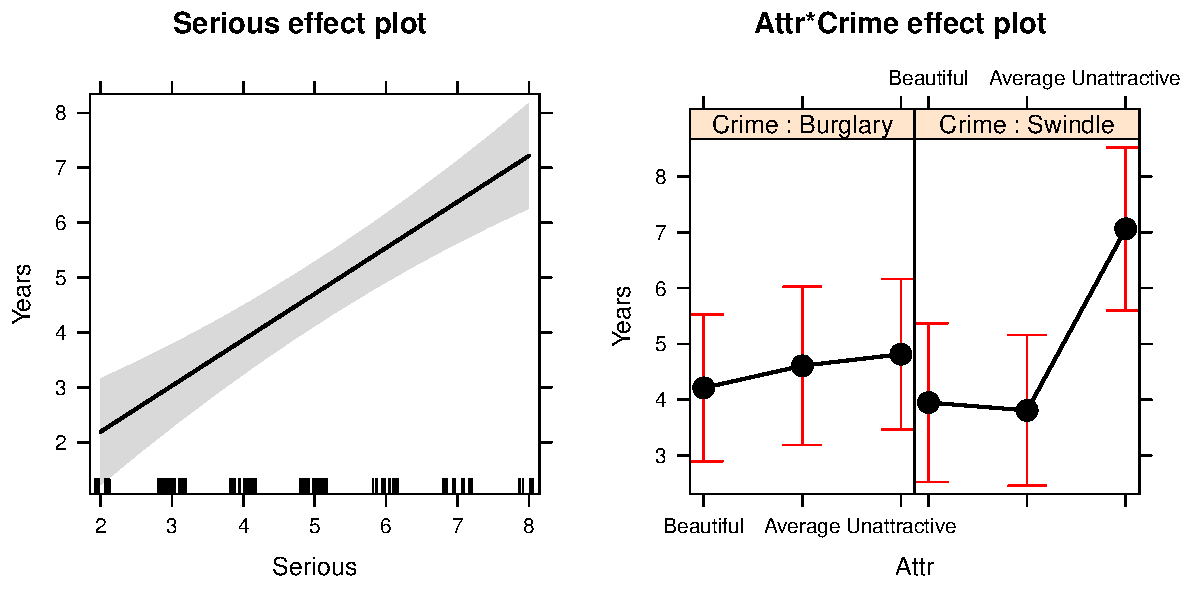
\includegraphics[width=\textwidth]{fig/plot-jury-mod3-eff}
\caption{Effect plots for  \code{Serious} and the \code{Attr * Crime}
	 in the ANCOVA model \code{jury.mod3}.}
\label{fig:jury-mod3-eff}
\end{center}
\end{figure}

The effect plot for \code{Serious} shows the expected linear relation
between that variable and \code{Years}. Of greater interest here is the nature
of the possible interaction of \code{Attr} and \code{Crime} on \code{Years}
of sentence, controlling for \code{Serious}.
The effect plot shows that for the crime of Swindle, there is a much
greater \code{Years} of sentence awarded to Unattractive defendents.

\subsection[Egyptian skulls]{Egyptian skulls from five epochs}
This example examines physical measurements of size and shape made on
150 Egyptian skulls from five epochs ranging from
4000 BC to 150 AD.
The measures are: maximal breadth (mb), basibregmatic height (bh),
basialveolar length (bl), and nasal height (nh) of each skull.
See \url{http://www.redwoods.edu/instruct/agarwin/anth_6_measurements.htm}
for the definitions of these measures, and \figref{fig:skulls} for a diagram.
The question of interest is whether and how these measurements change over time.
Systematic changes over time is of interest because this
would indicate interbreeding with immigrant populations.

\begin{figure}[htb]
\begin{center}
	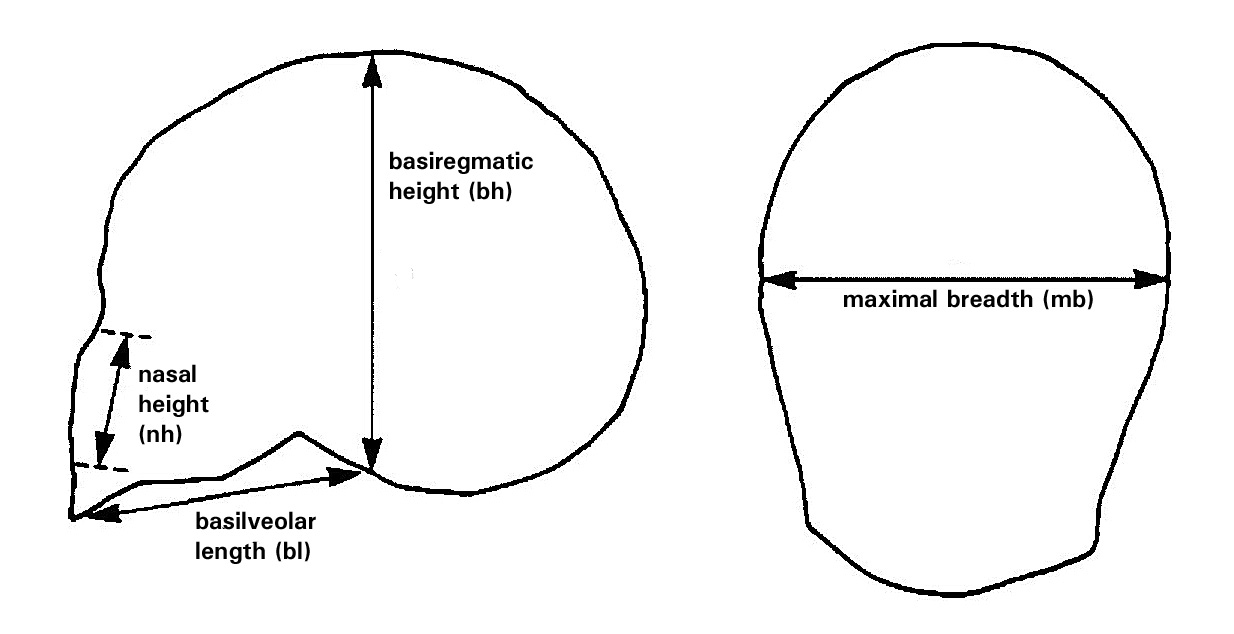
\includegraphics[width=.6\textwidth]{skulls}
\caption{Diagram of the skull measurements}
\label{fig:skulls}
\end{center}
\end{figure}


\begin{Schunk}
\begin{Sinput}
> data(Skulls)
> str(Skulls)
\end{Sinput}
\begin{Soutput}
'data.frame':	150 obs. of  5 variables:
 $ epoch: Ord.factor w/ 5 levels "c4000BC"<"c3300BC"<..: 1 1 1 1 1 1 1 1 1 1 ...
 $ mb   : num  131 125 131 119 136 138 139 125 131 134 ...
 $ bh   : num  138 131 132 132 143 137 130 136 134 134 ...
 $ bl   : num  89 92 99 96 100 89 108 93 102 99 ...
 $ nh   : num  49 48 50 44 54 56 48 48 51 51 ...
\end{Soutput}
\begin{Sinput}
> table(Skulls$epoch)
\end{Sinput}
\begin{Soutput}
c4000BC c3300BC c1850BC  c200BC  cAD150 
     30      30      30      30      30 
\end{Soutput}
\end{Schunk}
Note that \code{epoch} is an ordered factor, so the default contrasts
will be orthogonal polynomials.  This assumes that \code{epoch}
values are equally spaced, which they are not.  However, examining
the linear and quadratic trends is useful to a first approximation.

For ease of labeling various outputs, it is useful to trim the
\code{epoch} values and assign more meaningful variable labels.
\begin{Schunk}
\begin{Sinput}
> # make shorter labels for epochs
> Skulls$epoch <- factor(Skulls$epoch, labels=sub("c","",levels(Skulls$epoch)))
> # assign better variable labels
> vlab <- c("maxBreadth", "basibHeight", "basialLength", "nasalHeight")
\end{Sinput}
\end{Schunk}

We start with some simple displays of the means by epoch.  From the numbers,
the means don't seem to vary much.  
A \code{pairs} plot, \figref{fig:skulls4}, joining points
by \code{epoch} is somewhat more revealing for the bivariate relations among means.
\begin{Schunk}
\begin{Sinput}
> means <- aggregate(cbind(mb, bh, bl, nh) ~ epoch, data=Skulls, FUN=mean)[,-1]
> rownames(means) <- levels(Skulls$epoch)
> means
\end{Sinput}
\begin{Soutput}
           mb     bh     bl     nh
4000BC 131.37 133.60 99.167 50.533
3300BC 132.37 132.70 99.067 50.233
1850BC 134.47 133.80 96.033 50.567
200BC  135.50 132.30 94.533 51.967
AD150  136.17 130.33 93.500 51.367
\end{Soutput}
\end{Schunk}
\begin{Schunk}
\begin{Sinput}
> pairs(means, vlab,
        panel = function(x, y) {
            text(x, y, levels(Skulls$epoch))
            lines(x,y)
        })
\end{Sinput}
\end{Schunk}
\begin{figure}[htb]
\begin{center}
	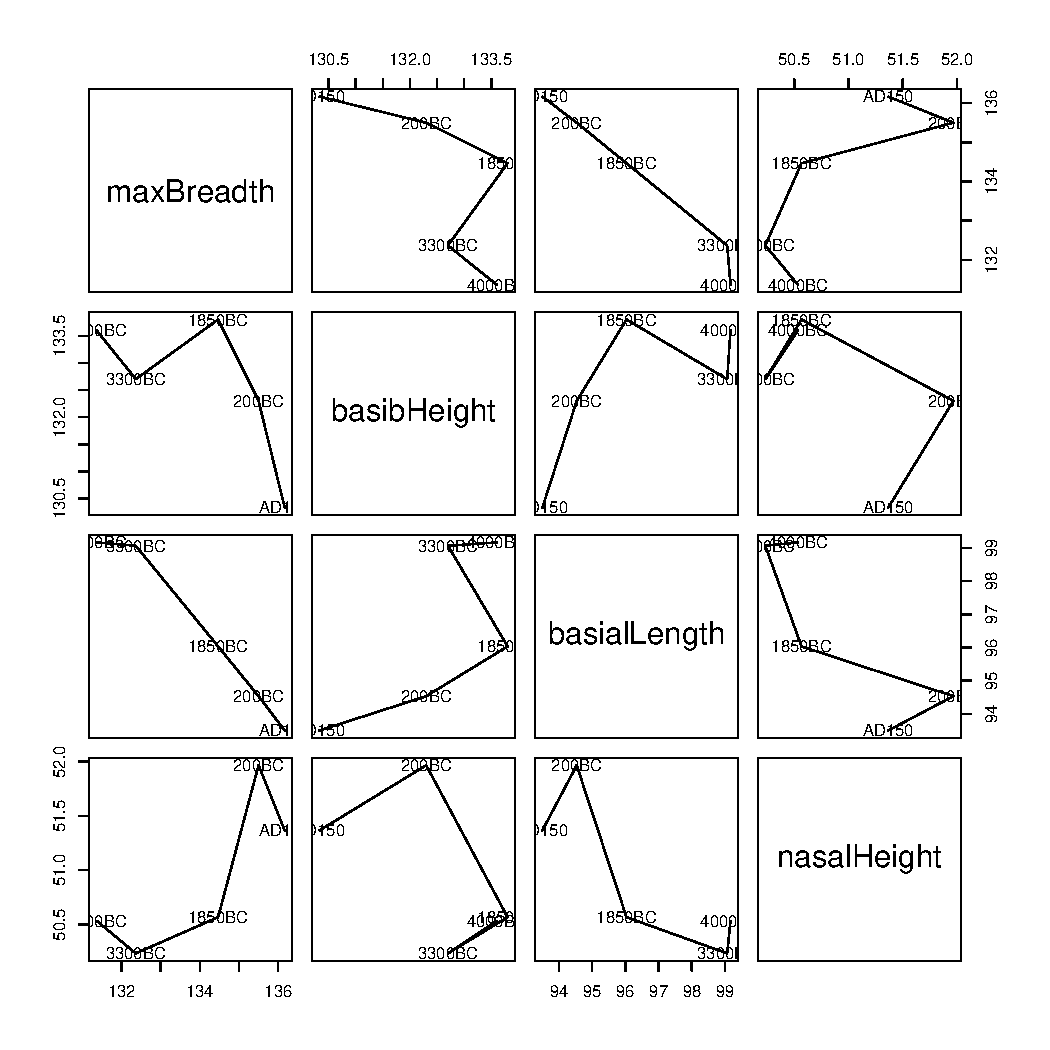
\includegraphics[width=.8\textwidth]{fig/plot-skulls4}
\caption{Pairs plot of means of Skulls data, by epoch}
\label{fig:skulls4}
\end{center}
\end{figure}

Perhaps better for visualizing the trends over time is a set of boxplots,
joining means over \code{epoch}. Using \func{bwplot} from the \pkg{lattice}
package requires reshaping the data from wide to long format.  The following
code produces \figref{fig:skulls-bwplot}.

\begin{Schunk}
\begin{Sinput}
> library(lattice)
> library(reshape2)
> sklong <- melt(Skulls, id="epoch")
> bwplot(value ~ epoch | variable, data=sklong, scales="free", 
  	ylab="Variable value", xlab="Epoch",
  	strip=strip.custom(factor.levels=paste(vlab, " (", levels(sklong$variable), ")", sep="")),
  	panel = function(x,y, ...) {
  		panel.bwplot(x, y, ...)
  		panel.linejoin(x,y, col="red", ...)
  	}) 
\end{Sinput}
\end{Schunk}
\begin{figure}[htb]
\begin{center}
	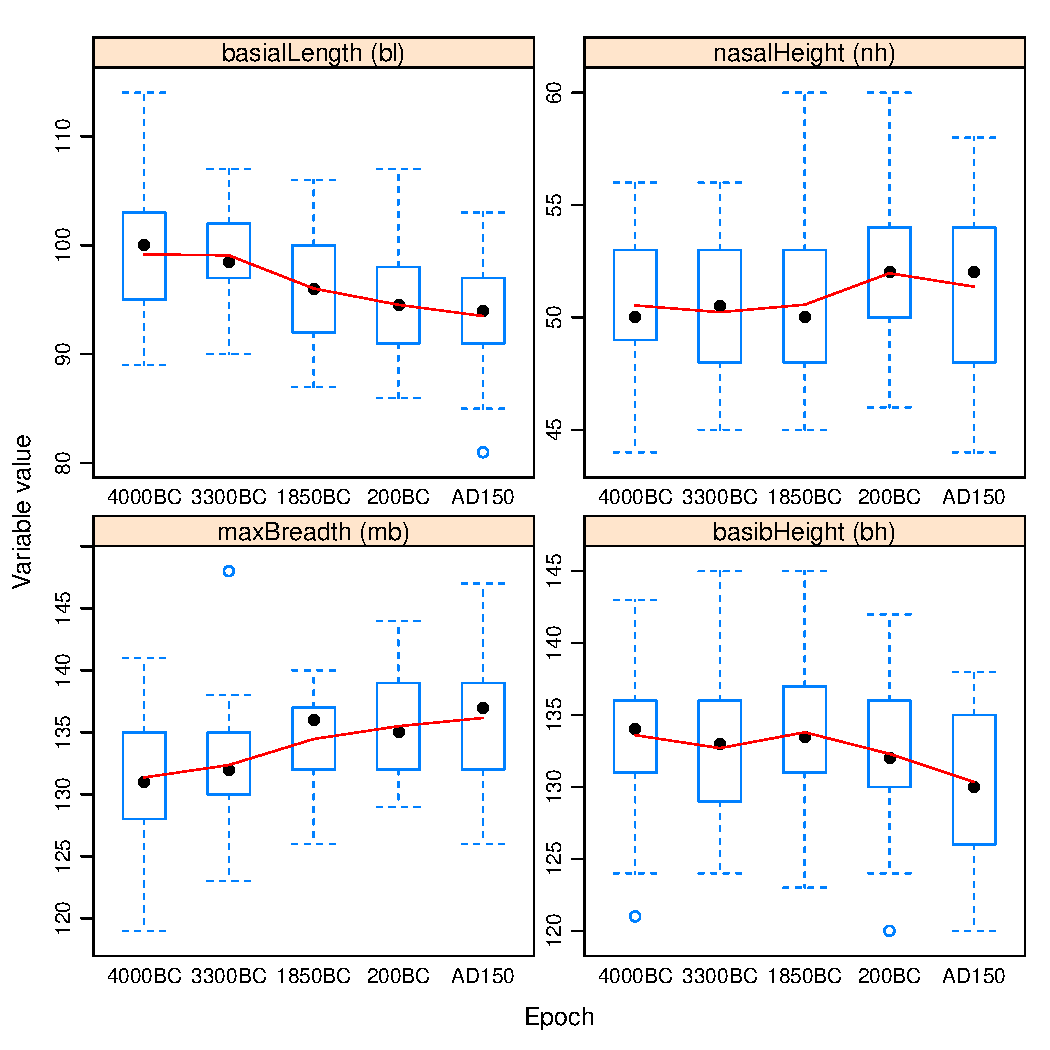
\includegraphics[width=.8\textwidth]{fig/plot-skulls-bwplot}
\caption{Boxplots of Skulls data, by epoch, for each variable}
\label{fig:skulls-bwplot}
\end{center}
\end{figure}

 
Now, fit the MANOVA model, and test the effect of \code{epoch} with \func{Manova}.
We see that the multivariate means differ substantially.
\begin{Schunk}
\begin{Sinput}
> # fit manova model
> sk.mod <- lm(cbind(mb, bh, bl, nh) ~ epoch, data=Skulls)
> Manova(sk.mod)
\end{Sinput}
\begin{Soutput}
Type II MANOVA Tests: Pillai test statistic
      Df test stat approx F num Df den Df  Pr(>F)    
epoch  4     0.353     3.51     16    580 4.7e-06 ***
---
Signif. codes:  0 '***' 0.001 '**' 0.01 '*' 0.05 '.' 0.1 ' ' 1 
\end{Soutput}
\end{Schunk}
Perhaps of greater interest are the more focused tests of trends over time.
These are based on tests of the coefficients in the model \code{sk.mod}
being jointly equal to zero, for subsets of the 
(polynomial) contrasts in \code{epoch}.
\begin{Schunk}
\begin{Sinput}
> coef(sk.mod)
\end{Sinput}
\begin{Soutput}
                   mb        bh        bl       nh
(Intercept) 133.97333 132.54667 96.460000 50.93333
epoch.L       4.02663  -2.19251 -5.017481  1.07517
epoch.Q      -0.46325  -1.26504 -0.089087  0.12472
epoch.C      -0.46380  -0.78003  1.075174 -0.83273
epoch^4       0.34263   0.80479 -0.661360 -0.41833
\end{Soutput}
\end{Schunk}

We use \func{linearHypothesis} for a multivariate test of the
\code{epoch.L} linear effect.
The linear trend is highly significant.  It is not obvious from 
\figref{fig:skulls4} that maximal breadth and nasal are increasing
over time, while the other two measurements have negative slopes.
\begin{Schunk}
\begin{Sinput}
> coef(sk.mod)["epoch.L",]
\end{Sinput}
\begin{Soutput}
     mb      bh      bl      nh 
 4.0266 -2.1925 -5.0175  1.0752 
\end{Soutput}
\begin{Sinput}
> print(linearHypothesis(sk.mod, "epoch.L"), SSP=FALSE) # linear component
\end{Sinput}
\begin{Soutput}
Multivariate Tests: 
                 Df test stat approx F num Df den Df    Pr(>F)    
Pillai            1   0.29138   14.597      4    142 5.195e-10 ***
Wilks             1   0.70862   14.597      4    142 5.195e-10 ***
Hotelling-Lawley  1   0.41119   14.597      4    142 5.195e-10 ***
Roy               1   0.41119   14.597      4    142 5.195e-10 ***
---
Signif. codes:  0 '***' 0.001 '**' 0.01 '*' 0.05 '.' 0.1 ' ' 1 
\end{Soutput}
\end{Schunk}
\func{linearHypothesis} can also be used to test composite hypotheses.
Here we test all non-linear coefficients jointly.  The result indicates
that, collectively, all non-linear terms are not significantly different
from zero.
\begin{Schunk}
\begin{Sinput}
> print(linearHypothesis(sk.mod, c("epoch.Q", "epoch.C", "epoch^4")), SSP=FALSE)
\end{Sinput}
\begin{Soutput}
Multivariate Tests: 
                 Df test stat approx F num Df den Df Pr(>F)
Pillai            3   0.06819  0.83726     12 432.00 0.6119
Wilks             3   0.93296  0.83263     12 375.99 0.6167
Hotelling-Lawley  3   0.07063  0.82791     12 422.00 0.6216
Roy               3   0.04519  1.62676      4 144.00 0.1707
\end{Soutput}
\end{Schunk}

Again, HE plots can show the patterns of these tests of multivariate hypotheses.
With four response variables, it is easiest to look at all pairwise
HE plots with the \func{pairs.mlm} function. 
The statement below produces \figref{fig:skulls-HE-pairs}.
In this plot, we show the hypothesis ellipsoids for the overall
effect of \code{epoch}, as well as those for the tests just shown
for the linear trend component \code{epoch.L}
as well as the joint test of all non-linear terms.
\begin{Schunk}
\begin{Sinput}
> pairs(sk.mod, variables = c(1, 4, 2, 3), hypotheses = list(Lin = "epoch.L", 
      NonLin = c("epoch.Q", "epoch.C", "epoch^4")), var.labels = vlab[c(1, 
      4, 2, 3)])
\end{Sinput}
\end{Schunk}

\begin{figure}[htb]
\begin{center}
	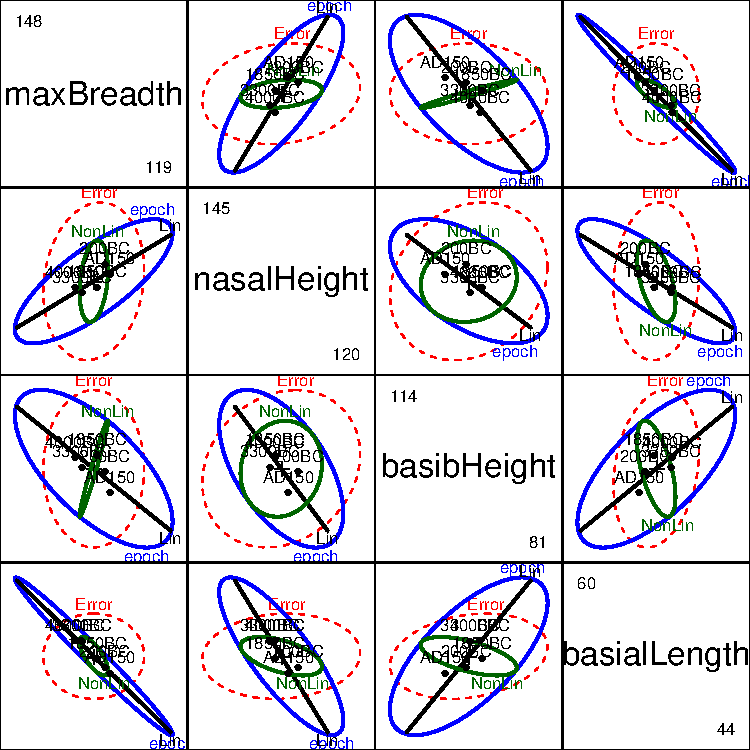
\includegraphics[width=.8\textwidth]{fig/plot-skulls-HE-pairs}
\caption{Pairs HE plot of Skulls data, showing multivariate tests of
	\code{epoch}, as well as tests of linear and nonlinear trends.}
\label{fig:skulls-HE-pairs}
\end{center}
\end{figure}
These plots have an interesting geometric interpretation:
the $\mat{H}$ ellipses for the overall effect of \code{epoch}
are representations of the additive decomposition of this effect into  
$\mat{H}$ ellipses for the linear and nonlinear linear
hypothesis tests according to
\begin{equation*}
	\mat{H}_{\textrm{epoch}} = \mat{H}_{\textrm{linear}} + \mat{H}_{\textrm{nonlinear}}
\end{equation*}
where the linear term has rank 1 (and so plots as a line), while the nonlinear
term has rank 3.  In each panel, it can be seen that the large direction of
the $\mat{H}_{\textrm{epoch}}$ leading to significance of this effect corresponds
essentially to the linear contrast.  $\mat{H}_{\textrm{nonlinear}}$ is the orthogonal
complement of $\mat{H}_{\textrm{linear}}$ in the space of $\mat{H}_{\textrm{epoch}}$,
but nowhere does it protrude beyond the boundary of the $\mat{E}$ ellipsoid.

These relations can be seen somewhat more easily in 3D, as produced using
\func{heplot3d} by the following statement.  The resulting plot is
better viewed interactively in R and is not reproduced here.
It would be seen there that the ellipsoid for the nonlinear terms
is nearly flat in one direction, corresponding to the panel for
(mb, hb) in \figref{fig:skulls-HE-pairs}.
\begin{Schunk}
\begin{Sinput}
> heplot3d(sk.mod, hypotheses=list(Lin="epoch.L", Quad="epoch.Q", 
                              NonLin=c("epoch.Q", "epoch.C", "epoch^4")), 
  	col=c("pink", "blue"))
\end{Sinput}
\end{Schunk}

Finally, a simpler view of these effects can be shown in the canonical
space corresponding to the canonical discriminant analysis for
\code{epoch}.  The computations are performed by \func{candisc}
which returns a class \code{"candisc"} object.

\begin{Schunk}
\begin{Sinput}
> library(candisc)
> sk.can <- candisc(sk.mod)
> sk.can
\end{Sinput}
\begin{Soutput}
Canonical Discriminant Analysis for epoch:

   CanRsq Eigenvalue Difference Percent Cumulative
1 0.29829    0.42510      0.386  88.227       88.2
2 0.03754    0.03900      0.386   8.094       96.3
3 0.01546    0.01570      0.386   3.259       99.6
4 0.00202    0.00202      0.386   0.419      100.0

Test of H0: The canonical correlations in the 
current row and all that follow are zero

  LR test stat approx F num Df den Df Pr(> F)    
1        0.664     3.90     16    434   7e-07 ***
2        0.946     0.90      9    348    0.53    
3        0.983     0.64      4    288    0.64    
4        0.998     0.29      1    145    0.59    
---
Signif. codes:  0 '***' 0.001 '**' 0.01 '*' 0.05 '.' 0.1 ' ' 1 
\end{Soutput}
\end{Schunk}
The output above shows that, although $\mat{H}_{\textrm{epoch}}$ is of rank 4,
two dimensions account for 96\% 
of the between-epoch variation.  By the likelihood ratio test, only
the canonical correlation for the first dimension can be considered
non-zero.

The canonical HE plot is produced by plotting the \code{sk.can} object,
giving \figref{fig:skulls-can2}.
\begin{Schunk}
\begin{Sinput}
> heplot(sk.can, prefix="Canonical dimension")
\end{Sinput}
\end{Schunk}
\begin{figure}[htb]
\begin{center}
	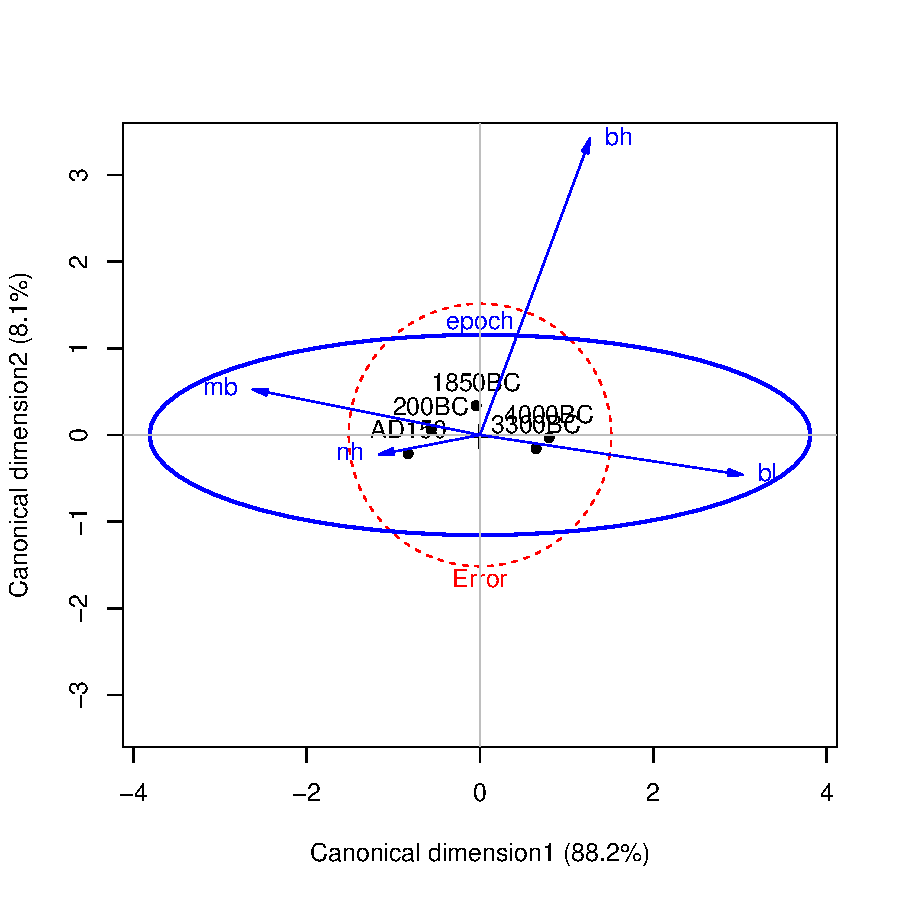
\includegraphics[width=.8\textwidth]{fig/plot-skulls-can2}
\caption{Canonical discriminant HE plot of the Skulls data}
\label{fig:skulls-can2}
\end{center}
\end{figure}
In this plot, the first canonical dimension (88\%) essentially
corresponds to the ordered values of \code{epoch}, from right to left.
The variable vectors for maximum breadth (mb), basialiveolar length (bl)
and nasal height (nh) are  largely aligned with this dimension, indicating that
they distinguish the groups of skulls according to time.  The lengths of these
vectors indicates their relative contribution to discrimination among the
group means.  Only the variable vector for basibregmatic height (bh)
points in the direction of the second canonical dimension, corresponding
to higher means in the middle of the range of epochs.  We leave it to
forensic anthropologists to determine if this has any meaning.
 
\section[MMRA Designs]{Multivariate Multiple Regression Designs}
The ideas behind HE plots extend naturally to multivariate multiple
regression (MMRA) and multivariate analysis of covariance (MANCOVA). 
In MMRA, the $\mat{X}$ matrix contains only quantitative predictors, while
in MANCOVA designs, there is a mixture of
factors and quantitative predictors (covariates).  

In the MANCOVA case,
there is often a subtle difference in emphasis:  true MANCOVA analyses focus on
the differences among groups defined by the factors, adjusting for 
(or controlling for) the quantitative covariates. Analyses concerned
with \emph{homogeneity of regression} focus on quantitative predictors
and attempt to test whether the regression relations are the same for
all groups defined by the factors.

\subsection{Rohwer data}

To illustrate the homogeneity of regression flavor,
we use data
from a study by Rohwer (given in Timm, 1975: Ex.\ 4.3, 4.7, and 4.23)\nocite%
{Timm:75} on kindergarten children, designed to determine how well a set of
paired-associate (PA) tasks predicted performance on the Peabody Picture
Vocabulary test (\texttt{PPVT}), a student achievement test (\texttt{SAT}),
and the Raven Progressive matrices test (\texttt{Raven}). The PA tasks
varied in how the stimuli were presented, and are called \emph{named} (%
\texttt{n}), \emph{still} (\texttt{s}), \emph{named still} (\texttt{ns}), 
\emph{named action} (\texttt{na}), and \emph{sentence still} (\texttt{ss}).

Two groups were tested: a group of $n=37$ children from a low socioeconomic
status (SES) school, and a group of $n=32$ high SES children from an
upper-class, white residential school. The data are in the data frame 
\texttt{Rohwer} in the \texttt{heplots} package:
\begin{Schunk}
\begin{Sinput}
> some(Rohwer,n=6)
\end{Sinput}
\begin{Soutput}
   group SES SAT PPVT Raven n  s ns na ss
14     1  Lo  30   55    13 2  1 12 20 17
17     1  Lo  19   66    13 7 12 21 35 27
18     1  Lo  45   54    10 0  6  6 14 16
21     1  Lo  32   48    16 0  7  9 14 18
37     1  Lo  79   54    14 0  6  6 15 14
57     2  Hi  99   94    16 4  6 14 27 19
\end{Soutput}
\end{Schunk}

At one extreme, we might be tempted to fit separate regression models for each
of the High and Low SES groups.  This approach is \emph{not} recommended because it
lacks power and does not allow hypotheses about equality of slopes and intercepts
to be tested directly.

\begin{Schunk}
\begin{Sinput}
> rohwer.ses1 <- lm(cbind(SAT, PPVT, Raven) ~ n + s + ns + na + ss, data=Rohwer, subset=SES=="Hi")
> Anova(rohwer.ses1)
\end{Sinput}
\begin{Soutput}
Type II MANOVA Tests: Pillai test statistic
   Df test stat approx F num Df den Df Pr(>F)   
n   1     0.202     2.02      3     24 0.1376   
s   1     0.310     3.59      3     24 0.0284 * 
ns  1     0.358     4.46      3     24 0.0126 * 
na  1     0.465     6.96      3     24 0.0016 **
ss  1     0.089     0.78      3     24 0.5173   
---
Signif. codes:  0 '***' 0.001 '**' 0.01 '*' 0.05 '.' 0.1 ' ' 1 
\end{Soutput}
\begin{Sinput}
> rohwer.ses2 <- lm(cbind(SAT, PPVT, Raven) ~ n + s + ns + na + ss, data=Rohwer, subset=SES=="Lo")
> Anova(rohwer.ses2)
\end{Sinput}
\begin{Soutput}
Type II MANOVA Tests: Pillai test statistic
   Df test stat approx F num Df den Df Pr(>F)  
n   1    0.0384     0.39      3     29  0.764  
s   1    0.1118     1.22      3     29  0.321  
ns  1    0.2252     2.81      3     29  0.057 .
na  1    0.2675     3.53      3     29  0.027 *
ss  1    0.1390     1.56      3     29  0.220  
---
Signif. codes:  0 '***' 0.001 '**' 0.01 '*' 0.05 '.' 0.1 ' ' 1 
\end{Soutput}
\end{Schunk}
This allows separate slopes and intercepts for each of the two groups, but it is difficult
to compare the coefficients numerically.
\begin{Schunk}
\begin{Sinput}
> coef(rohwer.ses1)
\end{Sinput}
\begin{Soutput}
                  SAT      PPVT     Raven
(Intercept) -28.46747 39.697090 13.243836
n             3.25713  0.067283  0.059347
s             2.99658  0.369984  0.492444
ns           -5.85906 -0.374380 -0.164022
na            5.66622  1.523009  0.118980
ss           -0.62265  0.410157 -0.121156
\end{Soutput}
\begin{Sinput}
> coef(rohwer.ses2)
\end{Sinput}
\begin{Soutput}
                  SAT      PPVT     Raven
(Intercept)  4.151060 33.005769 11.173378
n           -0.608872 -0.080567  0.210995
s           -0.050156 -0.721050  0.064567
ns          -1.732395 -0.298303  0.213584
na           0.494565  1.470418 -0.037318
ss           2.247721  0.323965 -0.052143
\end{Soutput}
\end{Schunk}
Nevertheless, we can visualize the results with HE plots, and here we make use of the fact
that several HE plots can be overlaid using the option \code{add=TRUE}
as shown in \figref{fig:rohwer-HE1}.
\begin{Schunk}
\begin{Sinput}
> heplot(rohwer.ses1, ylim=c(40,110),col=c("red", "black"), lwd=2, cex=1.2)
> heplot(rohwer.ses2, add=TRUE, col=c("blue", "black"), grand.mean=TRUE, error.ellipse=TRUE, lwd=2, cex=1.2)
> means <- aggregate(cbind(SAT,PPVT)~SES, data=Rohwer,  mean)
> text(means[,2], means[,3], labels=means[,1], pos=3, cex=2, col=c("red", "blue"))
\end{Sinput}
\end{Schunk}
\begin{figure}[htb]
\begin{center}
	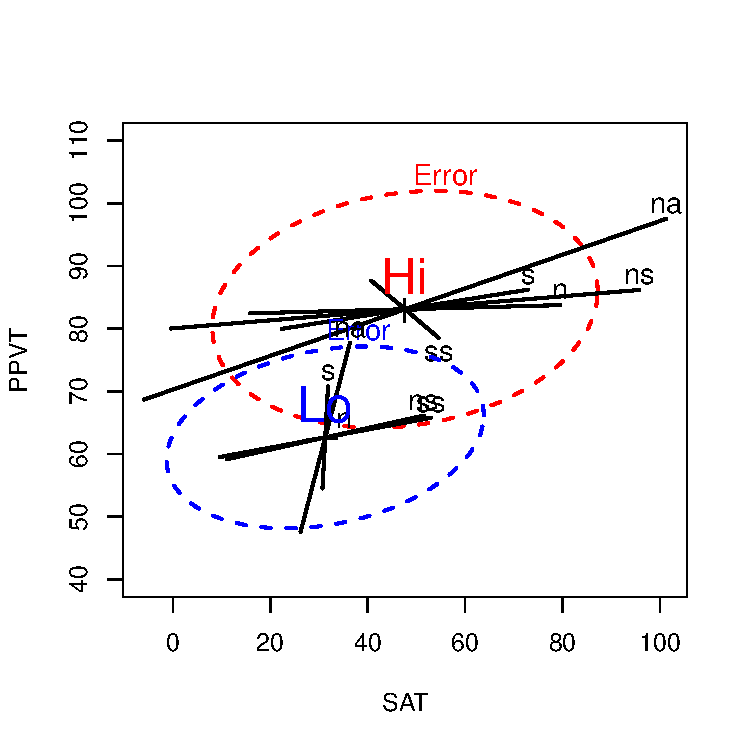
\includegraphics[width=.6\textwidth, trim=0 30 0 30]{fig/plot-rohwer-HE1}
\caption{HE plot for \code{SAT} and \code{PPVT}, showing the effects for the PA predictors
	for the High and Low SES groups separately}
\label{fig:rohwer-HE1}
\end{center}
\end{figure}

We can readily see the difference in means for the two SES groups (High greater on both variables)
and it also appears that the slopes of the predictor ellipses are shallower for the High
than the Low group, indicating greater relation with the \code{SAT} score. 

Alternatively (and optimistically), we can fit a MANCOVA model 
that allows different means for the two SES groups on the responses, but constrains the
slopes for the PA covariates to be equal.

\begin{Schunk}
\begin{Sinput}
> # MANCOVA, assuming equal slopes
> rohwer.mod <- lm(cbind(SAT, PPVT, Raven) ~ SES + n + s + ns + na + ss, 
                   data=Rohwer)
> Anova(rohwer.mod)
\end{Sinput}
\begin{Soutput}
Type II MANOVA Tests: Pillai test statistic
    Df test stat approx F num Df den Df  Pr(>F)    
SES  1     0.379    12.18      3     60 2.5e-06 ***
n    1     0.040     0.84      3     60  0.4773    
s    1     0.093     2.04      3     60  0.1173    
ns   1     0.193     4.78      3     60  0.0047 ** 
na   1     0.231     6.02      3     60  0.0012 ** 
ss   1     0.050     1.05      3     60  0.3770    
---
Signif. codes:  0 '***' 0.001 '**' 0.01 '*' 0.05 '.' 0.1 ' ' 1 
\end{Soutput}
\end{Schunk}

Note that, although the
multivariate tests for two of the covariates (\texttt{ns} and \texttt{na})
are highly significant, univariate multiple regression tests for the
separate responses [from \code{summary(rohwer.mod)}] are relatively weak.
We can also test the global 5 df hypothesis, $\mat{B}=\mat{0}$, 
that \emph{all} covariates have null effects
for all responses as a linear hypothesis (suppressing display of the error
and hypothesis SSP matrices),

\begin{Schunk}
\begin{Sinput}
> (covariates <- rownames(coef(rohwer.mod))[-(1:2)])
\end{Sinput}
\begin{Soutput}
[1] "n"  "s"  "ns" "na" "ss"
\end{Soutput}
\begin{Sinput}
> Regr<-linearHypothesis(rohwer.mod, covariates)
> print(Regr, digits=5, SSP=FALSE)
\end{Sinput}
\begin{Soutput}
Multivariate Tests: 
                 Df test stat approx F num Df den Df    Pr(>F)    
Pillai            5   0.66579   3.5369     15 186.00 2.309e-05 ***
Wilks             5   0.44179   3.8118     15 166.03 8.275e-06 ***
Hotelling-Lawley  5   1.03094   4.0321     15 176.00 2.787e-06 ***
Roy               5   0.75745   9.3924      5  62.00 1.062e-06 ***
---
Signif. codes:  0 '***' 0.001 '**' 0.01 '*' 0.05 '.' 0.1 ' ' 1 
\end{Soutput}
\end{Schunk}

Then 2D views of the
additive MANCOVA model \code{rohwer.mod} and the overall test for all covariates
are produced as follows, giving the plots in \figref{fig:rohwer-HE2}.
\begin{Schunk}
\begin{Sinput}
> colors <- c("red", "blue", rep("black",5), "#969696")
> heplot(rohwer.mod, col=colors,
        hypotheses=list("Regr" = c("n", "s", "ns", "na", "ss")),
        cex=1.5, lwd=c(2, rep(3,5), 4),
        main="(SAT, PPVT, Raven) ~ SES + n + s + ns + na + ss")
\end{Sinput}
\end{Schunk}
\begin{Schunk}
\begin{Sinput}
> heplot(rohwer.mod, col=colors,  variables=c(1,3),
        hypotheses=list("Regr" = c("n", "s", "ns", "na", "ss")),
        cex=1.5, lwd=c(2, rep(3,5), 4),
        main="(SAT, PPVT, Raven) ~ SES + n + s + ns + na + ss")
\end{Sinput}
\end{Schunk}

\begin{figure}[htb]
\begin{center}
	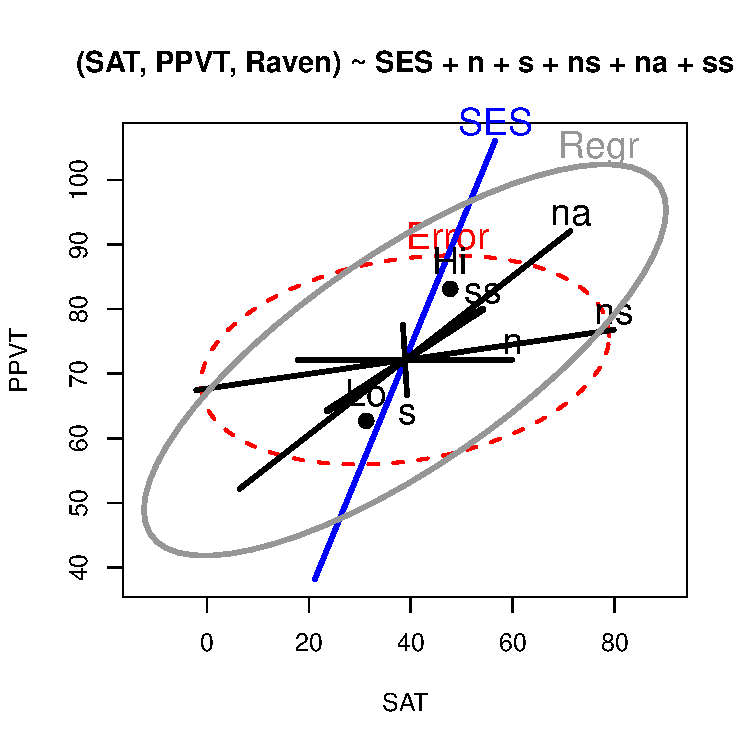
\includegraphics[width=.48\textwidth, trim=0 30 0 30]{fig/plot-rohwer-HE2}
	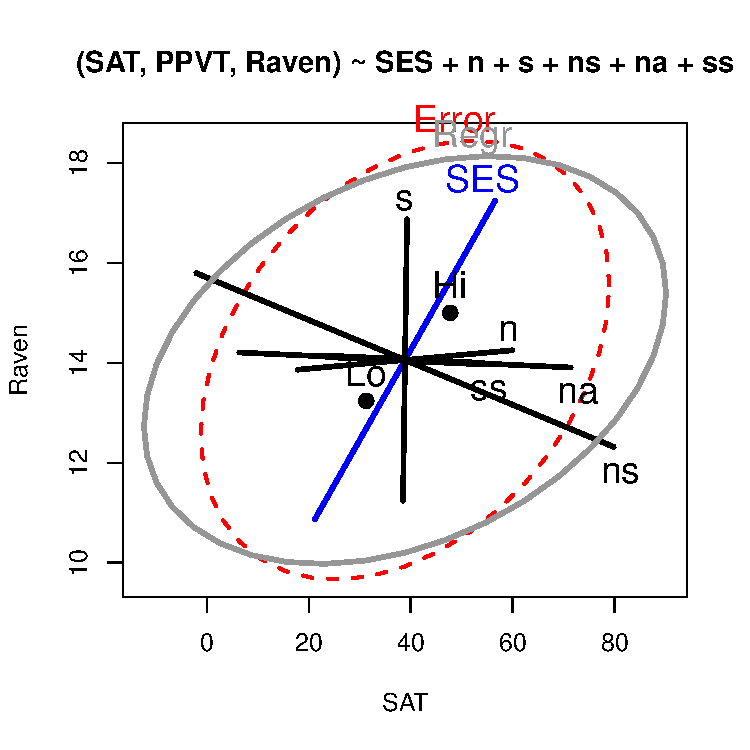
\includegraphics[width=.48\textwidth, trim=0 30 0 30]{fig/plot-rohwer-HE3}
\caption{HE plot for \code{SAT} and \code{PPVT} (left) and for 
	\code{SAT} and \code{Raven} (right) using the MANCOVA model }
\label{fig:rohwer-HE2}
\end{center}
\end{figure}

The positive orientation of the \code{Regr} ellipses shows that the prediced
values for all three responses are positively correlated (more so for
\code{SAT} and \code{PPVT}). As well, the High SES group
is higher on all responses than the Low SES group.

Alternatively, all pairwise plots among these responses could be drawn using
the \code{pairs} function (figure not shown),

\begin{Schunk}
\begin{Sinput}
> pairs(rohwer.mod, col=colors,
        hypotheses=list("Regr" = c("n", "s", "ns", "na", "ss")),
        cex=1.3, lwd=c(2, rep(3,5), 4))
\end{Sinput}
\end{Schunk}
or as a 3D plot, using \func{heplot3d} as shown in \figref{fig:rohwer-HE3D}.
\begin{Schunk}
\begin{Sinput}
> colors <- c("pink", "blue", rep("black",5), "#969696")
> heplot3d(rohwer.mod, col=colors,
  	hypotheses=list("Regr" = c("n", "s", "ns", "na", "ss")))
\end{Sinput}
\end{Schunk}
\begin{figure}[htb]
\begin{center}
	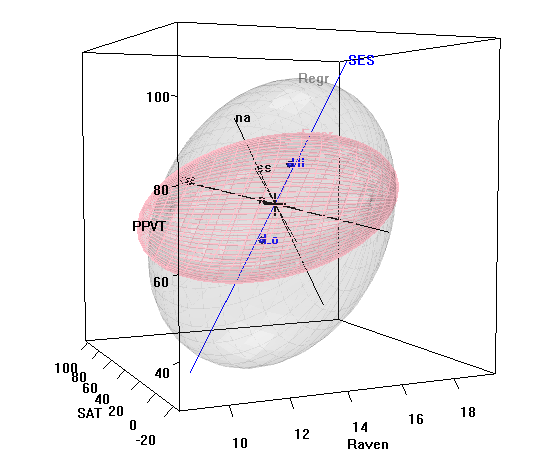
\includegraphics[width=.6\textwidth]{rohwer-HE3D}
\caption{3D HE plot for the MANCOVA model fit to the Rohwer data}
\label{fig:rohwer-HE3D}
\end{center}
\end{figure}

The MANCOVA model, \code{rohwer.mod}, has relatively simple interpretations
(large effect of \code{SES}, with \code{ns} and \code{na} as the major predictors)
but the test of relies on the assumption of homogeneity of slopes for the predictors.
We can test this as follows, adding interactions of \code{SES}
with each of the covariates:

\begin{Schunk}
\begin{Sinput}
> rohwer.mod2 <- lm(cbind(SAT, PPVT, Raven) ~ SES * (n + s + ns + na + ss),
                    data=Rohwer)
> Anova(rohwer.mod2)
\end{Sinput}
\begin{Soutput}
Type II MANOVA Tests: Pillai test statistic
       Df test stat approx F num Df den Df  Pr(>F)    
SES     1     0.391    11.78      3     55 4.5e-06 ***
n       1     0.079     1.57      3     55 0.20638    
s       1     0.125     2.62      3     55 0.05952 .  
ns      1     0.254     6.25      3     55 0.00100 ***
na      1     0.307     8.11      3     55 0.00015 ***
ss      1     0.060     1.17      3     55 0.32813    
SES:n   1     0.072     1.43      3     55 0.24417    
SES:s   1     0.099     2.02      3     55 0.12117    
SES:ns  1     0.118     2.44      3     55 0.07383 .  
SES:na  1     0.148     3.18      3     55 0.03081 *  
SES:ss  1     0.057     1.12      3     55 0.35094    
---
Signif. codes:  0 '***' 0.001 '**' 0.01 '*' 0.05 '.' 0.1 ' ' 1 
\end{Soutput}
\end{Schunk}
It appears from the above that there is only weak evidence of unequal slopes
from the separate \code{SES:} terms. The evidence for heterogeneity is
stronger, however, when these terms are tested collectively using the 
\func{linearHypothesis} function:

\begin{Schunk}
\begin{Sinput}
> (coefs <- rownames(coef(rohwer.mod2)))
\end{Sinput}
\begin{Soutput}
 [1] "(Intercept)" "SESLo"       "n"           "s"           "ns"         
 [6] "na"          "ss"          "SESLo:n"     "SESLo:s"     "SESLo:ns"   
[11] "SESLo:na"    "SESLo:ss"   
\end{Soutput}
\begin{Sinput}
> print(linearHypothesis(rohwer.mod2, coefs[grep(":", coefs)]), SSP=FALSE)
\end{Sinput}
\begin{Soutput}
Multivariate Tests: 
                 Df test stat approx F num Df den Df   Pr(>F)   
Pillai            5   0.41794   1.8452     15 171.00 0.032086 * 
Wilks             5   0.62358   1.8936     15 152.23 0.027695 * 
Hotelling-Lawley  5   0.53865   1.9272     15 161.00 0.023962 * 
Roy               5   0.38465   4.3850      5  57.00 0.001905 **
---
Signif. codes:  0 '***' 0.001 '**' 0.01 '*' 0.05 '.' 0.1 ' ' 1 
\end{Soutput}
\end{Schunk}
This model (\code{rohwer.mod2}) is similar in spirit to the two models
(\code{rohwer.ses1} and \code{rohwer.ses2})
fit for the two SES groups separately and show in \figref{fig:rohwer-HE1},
except that model \code{rohwer.mod2} assumes a common within-groups error covariance matrix
and allows overall tests.

To illustrate model \code{rohwer.mod2}, we construct an HE plot for
\code{SAT} and \code{PPVT} shown in \figref{fig:rohwer-HE4}. 
To simplify this display, we show the hypothesis ellipses\
for the overall effects of the PA tests in the baseline high-SES group, and
a single combined ellipse for all the \texttt{SESLo:} interaction terms that
we tested previously, representing differences in slopes between the low and
high-SES groups. 

Because SES is ``treatment-coded'' in this model, the ellipse for each
covariate represents the hypothesis that the slopes for that covariate are
zero in the high-SES baseline category.  With this parameterization, the ellipse for
\code{Slopes} represents the joint hypothesis that slopes for the covariates do not differ
in the low-SES group. 

\begin{Schunk}
\begin{Sinput}
> colors <- c("red", "blue", rep("black",5), "#969696")
> heplot(rohwer.mod2, col=c(colors, "brown"), 
        terms=c("SES", "n", "s", "ns", "na", "ss"), 
        hypotheses=list("Regr" = c("n", "s", "ns", "na", "ss"),
                        "Slopes" = coefs[grep(":", coefs)]))
\end{Sinput}
\end{Schunk}
\begin{figure}[htb]
\begin{center}
	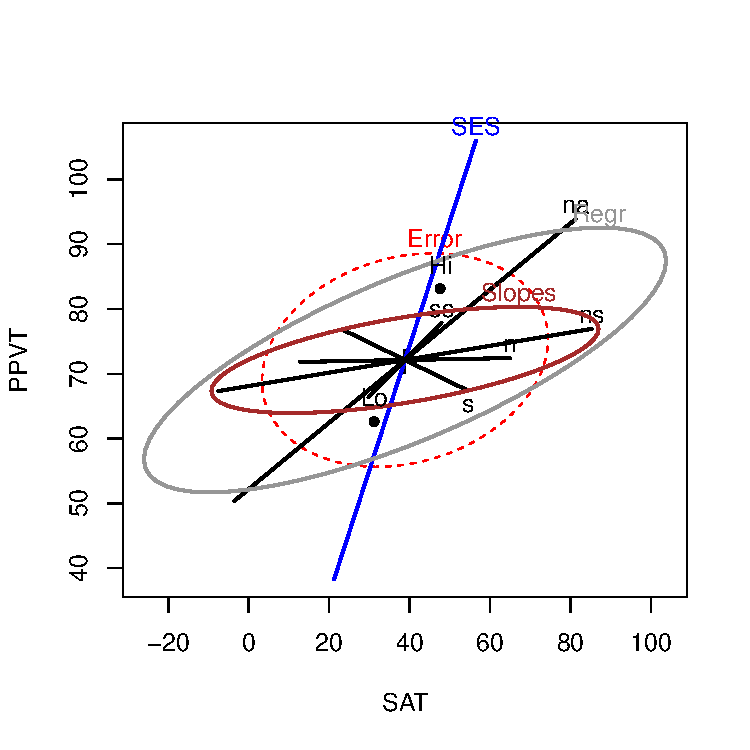
\includegraphics[width=.6\textwidth, trim=0 30 0 30]{fig/plot-rohwer-HE4}
\caption{HE plot for \code{SAT} and \code{PPVT}, fitting the model \code{rohwer.mod2}
	that allows unequal slopes for the covariates.  }
\label{fig:rohwer-HE4}
\end{center}
\end{figure}

Comparing \figref{fig:rohwer-HE4} for the heterogeneous slopes model
with \figref{fig:rohwer-HE2} (left) for the homogeneous slopes model,
it can be seen that most of the covariates have ellipses of similar
size and orientation, reflecting simlar evidence against the respective
null hypotheses, as does the effect of \code{SES}, showing the
greater performance of the high-SES group on all response measures.
Somewhat more subtle, the error ellipse is noticeably smaller in
\figref{fig:rohwer-HE4}, reflecting the additional variation accounted
for by differences in slopes.

\subsection[Hernior data]{Recovery from hernia repair}
This example uses the \code{Hernior} data, comprising
data on measures of post-operative recovery of 32 patients undergoing an
elective herniorrhaphy operation, in relation to pre-operative measures.

The response measures are
the patient's condition upon leaving the recovery room 
(\code{leave}, a 1-4 scale, 1=best),
level of nursing required one week after operation
(\code{nurse}, a 1-5 scale, 1=worst) and 
length of stay in hospital after operation (\code{los}, in days)

The predictor variables are patient \code{age}, \code{sex},
physical status (\code{pstat}, a 1-5 scale, with 1=perfect health, 5=very poor health),
body build (\code{build}, a 1-5 scale, with 1=emaciated, \dots, 5=obsese),
and preoperative complications with (\code{cardiac}) heart and respiration (\code{resp}).

We begin with a model fitting all predictors. Note that the ordinal predictors,
\code{pstat}, \code{build}, \code{cardiac} and \code{resp} could arguably be treated as
factors, rather than linear, regression terms.  We ignore this possibility in this example.

\begin{Schunk}
\begin{Sinput}
> Hern.mod <- lm(cbind(leave, nurse, los) ~ age + sex +  pstat +  build + cardiac + resp, 
                 data=Hernior)
> Anova(Hern.mod) 
\end{Sinput}
\begin{Soutput}
Type II MANOVA Tests: Pillai test statistic
        Df test stat approx F num Df den Df Pr(>F)  
age      1     0.143     1.27      3     23  0.307  
sex      1     0.026     0.21      3     23  0.892  
pstat    1     0.333     3.84      3     23  0.023 *
build    1     0.257     2.65      3     23  0.073 .
cardiac  1     0.228     2.26      3     23  0.108  
resp     1     0.248     2.53      3     23  0.082 .
---
Signif. codes:  0 '***' 0.001 '**' 0.01 '*' 0.05 '.' 0.1 ' ' 1 
\end{Soutput}
\end{Schunk}
The results of the multivariate tests above are somewhat disappointing.  Only the physical status
predictor (\code{pstat}) appears to be significant at conventional levels.

The univariate models for each response are implicit in the \MLM\ \code{Hern.mod}.
These can be printed using \func{summary}, or we can use \func{summary} to extract
certain statistics for each univariate response model, as we do here.

\begin{Schunk}
\begin{Sinput}
> Hern.summary <- summary(Hern.mod)
> unlist(lapply(Hern.summary, function(x) x$r.squared))
\end{Sinput}
\begin{Soutput}
Response leave Response nurse   Response los 
       0.59176        0.24740        0.36531 
\end{Soutput}
\end{Schunk}
The univariate tests for predictors in each of these models (not shown here)
are hard to interpret, and largely show only significant effects for 
the \code{leave} variable.  Yet, the $R^2$ values for the other responses
are slightly promising.  We proceed to an overall test of $\mat{B} = 0$
for all predictors.

\begin{Schunk}
\begin{Sinput}
> # test overall regression
> Regr <- linearHypothesis(Hern.mod, c("age", "sexm", "pstat", "build", "cardiac", "resp"))
> print(Regr, digits=5, SSP=FALSE)
\end{Sinput}
\begin{Soutput}
Multivariate Tests: 
                 Df test stat approx F num Df den Df    Pr(>F)    
Pillai            6   1.10198   2.4192     18 75.000 0.0041356 ** 
Wilks             6   0.21734   2.6046     18 65.539 0.0025239 ** 
Hotelling-Lawley  6   2.26797   2.7300     18 65.000 0.0016285 ** 
Roy               6   1.55434   6.4764      6 25.000 0.0003232 ***
---
Signif. codes:  0 '***' 0.001 '**' 0.01 '*' 0.05 '.' 0.1 ' ' 1 
\end{Soutput}
\end{Schunk}

\begin{Schunk}
\begin{Sinput}
> clr <- c("red", "darkgray", "blue", "darkgreen", "magenta", "brown", "black")
> vlab <- c("LeaveCondition\n(leave)", "NursingCare\n(nurse)", "LengthOfStay\n(los)")
> hyp <- list("Regr" = c("age", "sexm", "pstat", "build", "cardiac", "resp"))
> pairs(Hern.mod, hypotheses=hyp, col=clr, var.labels=vlab)
\end{Sinput}
\end{Schunk}

\begin{figure}[htb]
\begin{center}
	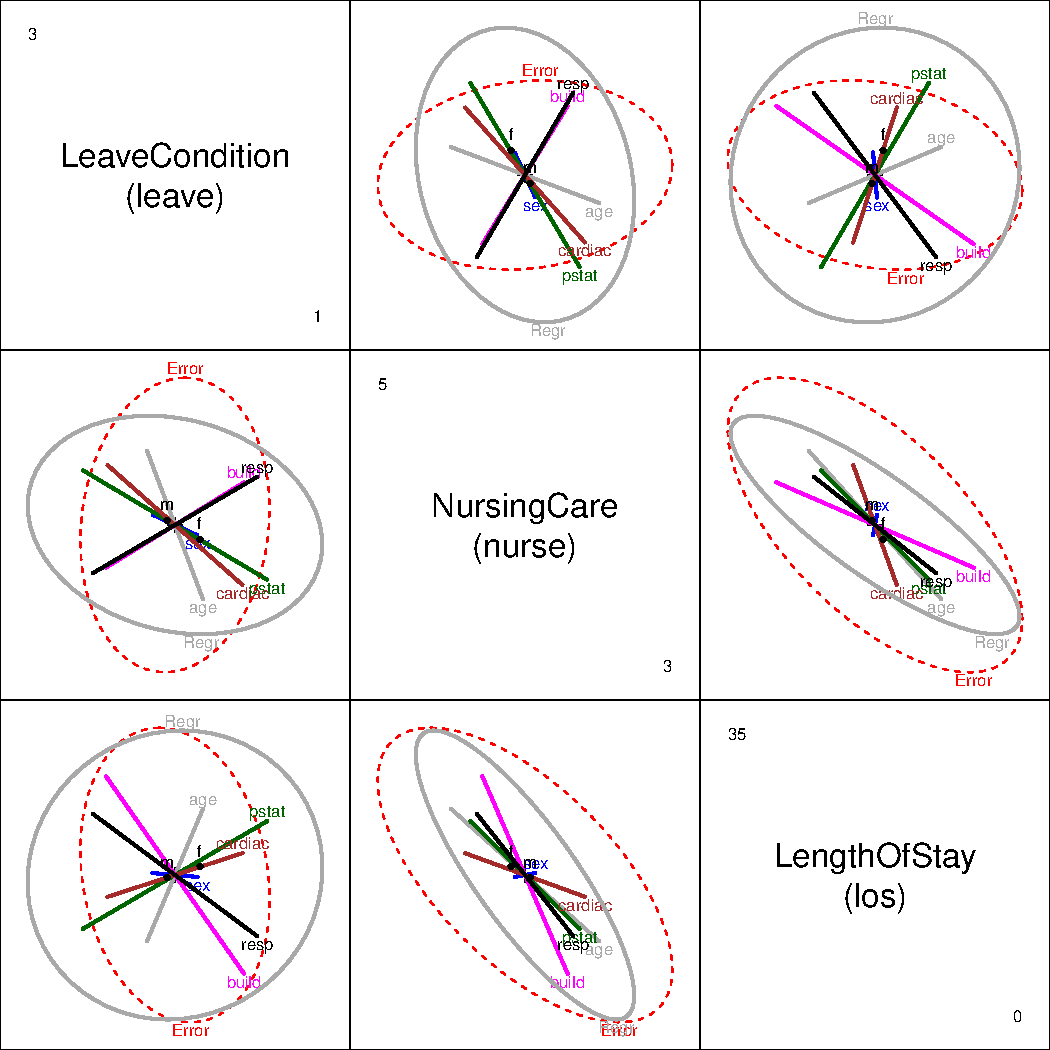
\includegraphics[width=.8\textwidth]{fig/plot-hern-pairs}
\caption{HE pairs plot for Hernior data}
\label{fig:hern-pairs}
\end{center}
\end{figure}

A \func{pairs} plot for the \MLM gives the set of plots shown in \figref{fig:hern-pairs}
helps to interpret the relations among the predictors which lead to the highly significant
overall test.
Among the predictors, age and sex have small and insignificant effects on the outcome measures
jointly.  The other predictors all contribute to the overall test of $\mat{B} = 0$,
though in different ways for the various responses.
For example, in the panel for (\code{leave}, \code{los}) in  \figref{fig:hern-pairs},
it can be seen that while only \code{pstat} individually is outside the 
$\mat{E}$ ellipse, \code{build} and \code{resp} contribute to the overall test in
an opposite direction.
 
In this multivariate regression example, all of the terms in the model \code{Hern.mod}
have 1 df, and so plot as lines in HE plots.  An alternative view of these effects
can be seen in canonical discriminant space, which, for each predictor shows the
scores on the linear combination of the responses that contributes most to 
the multivariate test of that effect, together with the weights for the responses.
We use \func{candiscList} to calculate the canonical analyses for all terms in
\code{Hern.mod}.
\begin{Schunk}
\begin{Sinput}
> Hern.canL <- candiscList(Hern.mod)
\end{Sinput}
\end{Schunk}

1D canonical discriminant plots for all terms can be obtained interactively 
with a menu, simply by plotting the \code{Hern.canL} object.
\begin{Schunk}
\begin{Sinput}
> plot(Hern.canL)
\end{Sinput}
\end{Schunk}
Plots for separate terms are produced by the lines below, and shown in 
\figref{fig:hern-can1} and \figref{fig:hern-can2}.
\begin{Schunk}
\begin{Sinput}
> plot(Hern.canL, term="pstat")
> plot(Hern.canL, term="build")
> plot(Hern.canL, term="age")
> plot(Hern.canL, term="cardiac")
\end{Sinput}
\end{Schunk}

\begin{figure}[htb]
\begin{center}
	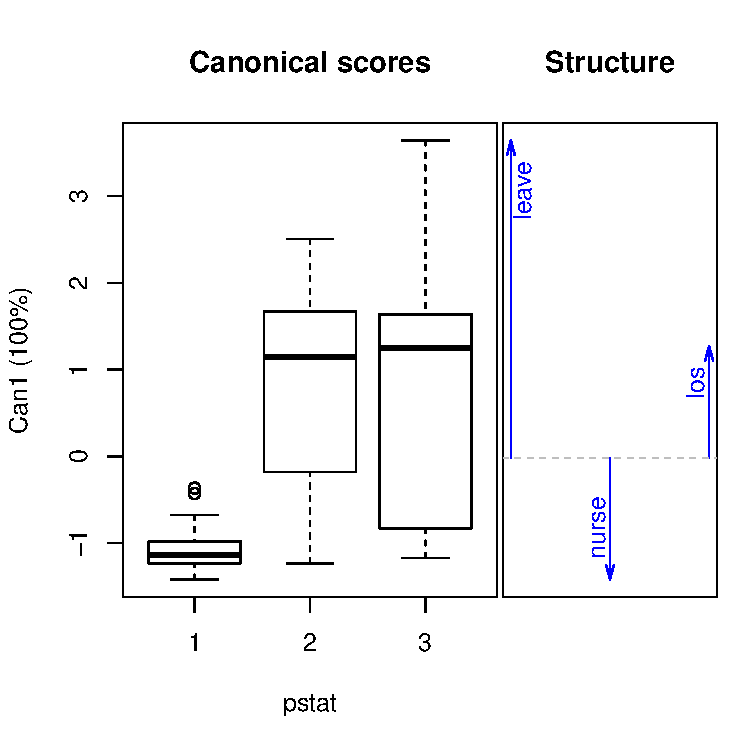
\includegraphics[width=.48\textwidth]{fig/plot-hern-can-pstat}
	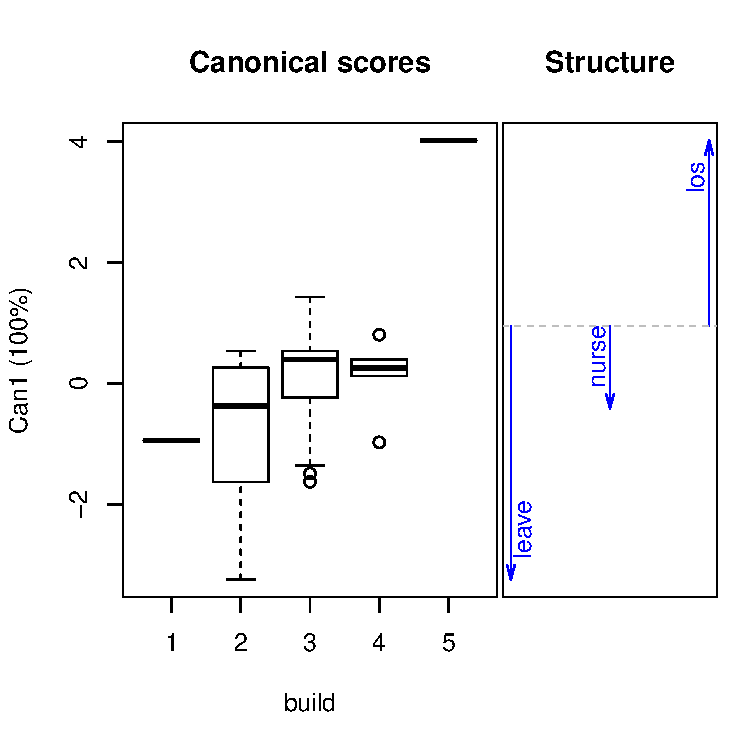
\includegraphics[width=.48\textwidth]{fig/plot-hern-can-build}
\caption{1D Canonical discriminant plots for \code{pstat} and \code{build}.
	The canonical scores are such that better outcomes are associated with smaller scores.}
\label{fig:hern-can1}
\end{center}
\end{figure}

\begin{figure}[htb!]
\begin{center}
	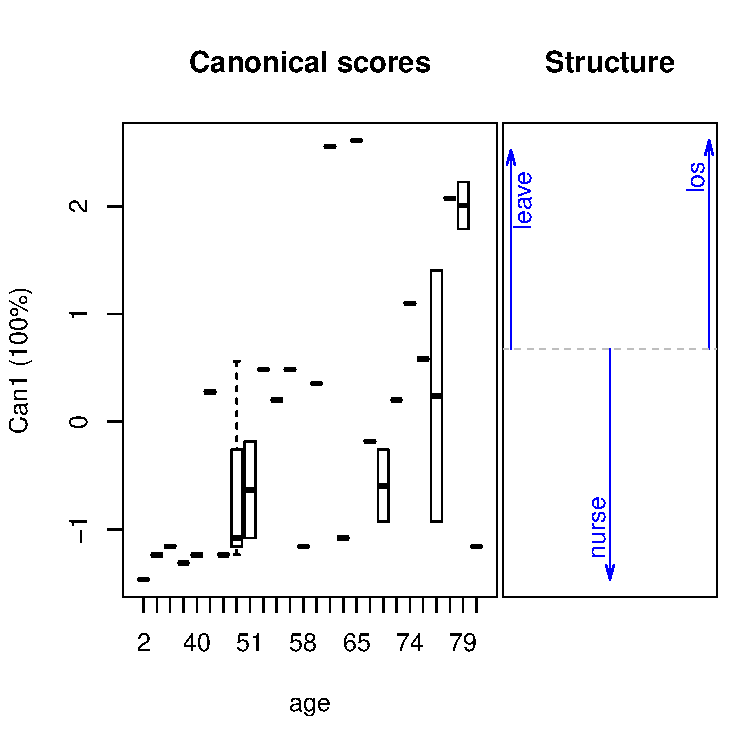
\includegraphics[width=.48\textwidth]{fig/plot-hern-can-age}
	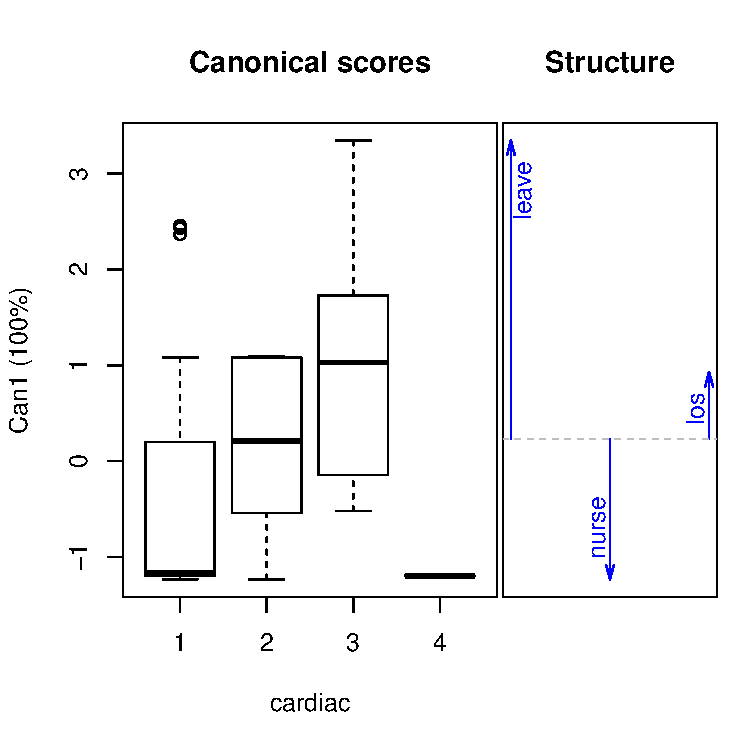
\includegraphics[width=.48\textwidth]{fig/plot-hern-can-cardiac}
\caption{1D Canonical discriminant plots for \code{age} and \code{cardiac}.
	}
\label{fig:hern-can2}
\end{center}
\end{figure}

In these plots, the canonical scores panel shows
the linear combinations of the
response variables which have the largest possible $R^2$.
Better outcomes correspond to numerically smaller canonical scores.
The arrows in the structure panel are proportional to
the canonical weights.

These plots provide simple interpretations of the results for the
canonical combinations of the responses.
Better physical status, smaller body build, lower age and absence
of cardiac complications are all positively related to better outcomes.
	
%\SweaveInput{SocGrades.Rnw}

\subsection[SocGrades]{Grades in a Sociology Course}

The data set \code{SocGrades} contains four outcome measures on student performance
in an introductory sociology course together with six potential predictors.
These data were used by Marascuilo and Levin (1983) for an example of
canonical correlation analysis, but are also suitable as examples of
multivariate multiple regression, MANOVA, MANCOVA
and step-down analysis in multivariate linear models.

The outcome measures used here are three test scores during the course,
\code{midterm1}, \code{midterm2}, \code{final},
and a course evaluation (\code{eval}).%
\footnote{It is arguable that the students' course evaluation should not
	be considered a response variable here.  It could be used as a
	predictor in a follow-up, 	step-down analysis, which would address the separate
	question of
	whether the effects on exam grades remain, when \code{eval} is 
	controlled for.  
}
Predictor variables are student's social class (\code{class}, an ordered factor with levels \code{1} > \code{2} > \code{3})
  \code{sex},
  grade point average (\code{gpa}),
  College Board test scores (\code{boards}),
  previous high school unit in sociology?  (\code{hssoc}: \code{no}, \code{yes}), and
  score on a course pretest (\code{pretest}).

The basic \MLM\ is fit below as \code{grades.mod}.
\begin{Schunk}
\begin{Sinput}
> data(SocGrades)
> grades.mod <- lm(cbind(midterm1, midterm2, final, eval) ~ 
  	class + sex + gpa + boards + hssoc + pretest, data=SocGrades)
> Anova(grades.mod, test="Roy")
\end{Sinput}
\begin{Soutput}
Type II MANOVA Tests: Roy test statistic
        Df test stat approx F num Df den Df  Pr(>F)    
class    2     1.567    11.75      4     30 7.3e-06 ***
sex      1     0.553     4.01      4     29  0.0104 *  
gpa      1     1.208     8.76      4     29 9.2e-05 ***
boards   1     0.731     5.30      4     29  0.0025 ** 
hssoc    1     0.035     0.25      4     29  0.9052    
pretest  1     0.313     2.27      4     29  0.0859 .  
---
Signif. codes:  0 '***' 0.001 '**' 0.01 '*' 0.05 '.' 0.1 ' ' 1 
\end{Soutput}
\end{Schunk}

In both univariate and multivariate
response models, it is often useful to screen for higher-order
terms (interactions, non-linear predictors).  This can most easily be
done using \func{update}, as we do below.  First, try the extended
model with all pairwise interactions of the predictors.

\begin{Schunk}
\begin{Sinput}
> grades.mod2 <- update(grades.mod, . ~ .^2)
> Anova(grades.mod2, test="Roy")
\end{Sinput}
\begin{Soutput}
Type II MANOVA Tests: Roy test statistic
               Df test stat approx F num Df den Df Pr(>F)   
class           2     2.817     7.04      4     10 0.0058 **
sex             1     0.487     1.09      4      9 0.4152   
gpa             1     1.998     4.49      4      9 0.0286 * 
boards          1     2.338     5.26      4      9 0.0183 * 
hssoc           1     0.281     0.63      4      9 0.6522   
pretest         1     0.510     1.15      4      9 0.3946   
class:sex       2     2.039     5.10      4     10 0.0168 * 
class:gpa       2     0.982     2.45      4     10 0.1137   
class:boards    2     0.522     1.31      4     10 0.3321   
class:hssoc     2     0.356     0.89      4     10 0.5041   
class:pretest   2     1.005     2.51      4     10 0.1082   
sex:gpa         1     0.269     0.60      4      9 0.6694   
sex:boards      1     0.184     0.41      4      9 0.7944   
sex:hssoc       1     0.909     2.04      4      9 0.1714   
sex:pretest     1     0.885     1.99      4      9 0.1795   
gpa:boards      1     0.447     1.00      4      9 0.4537   
gpa:hssoc       1     0.596     1.34      4      9 0.3269   
gpa:pretest     1     0.472     1.06      4      9 0.4291   
boards:hssoc    1     0.353     0.80      4      9 0.5573   
boards:pretest  1     0.705     1.59      4      9 0.2593   
hssoc:pretest   1     1.464     3.29      4      9 0.0635 . 
---
Signif. codes:  0 '***' 0.001 '**' 0.01 '*' 0.05 '.' 0.1 ' ' 1 
\end{Soutput}
\end{Schunk}
In the results above, only the interaction of \code{class:sex} is significant,
and the main effects of \code{hssoc} and \code{pretest} remain insignificant.
A revised model to explore is \code{grades.mod3},

\begin{Schunk}
\begin{Sinput}
> grades.mod3 <- update(grades.mod, . ~ . + class:sex - hssoc - pretest)
> Anova(grades.mod3, test="Roy")
\end{Sinput}
\begin{Soutput}
Type II MANOVA Tests: Roy test statistic
          Df test stat approx F num Df den Df  Pr(>F)    
class      2     1.588    11.91      4     30 6.5e-06 ***
sex        1     0.575     4.17      4     29 0.00864 ** 
gpa        1     1.434    10.40      4     29 2.4e-05 ***
boards     1     0.895     6.49      4     29 0.00074 ***
class:sex  2     0.450     3.38      4     30 0.02143 *  
---
Signif. codes:  0 '***' 0.001 '**' 0.01 '*' 0.05 '.' 0.1 ' ' 1 
\end{Soutput}
\end{Schunk}

A pairwise HE plot for all responses (\figref{fig:grades-pairs}) shows that nearly all 
effects are in the expected directions: higher \code{gpa}, \code{boards}, \code{class}
leads to better performance on most outcomes.  The interaction of
\code{class:sex} seems to be confined largely to \code{midterm1}.
\begin{Schunk}
\begin{Sinput}
> pairs(grades.mod3)
\end{Sinput}
\end{Schunk}

\begin{figure}[htb]
\begin{center}
	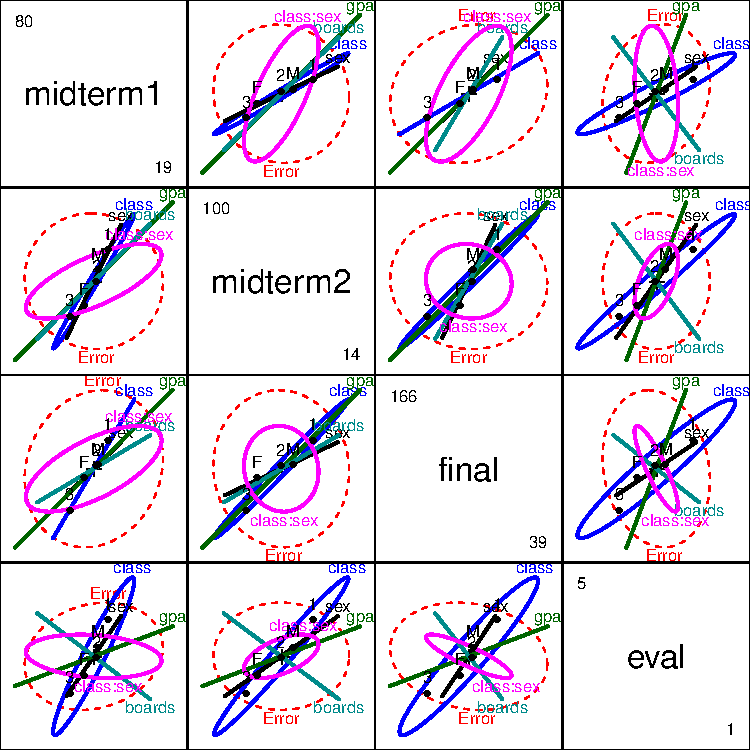
\includegraphics[width=.8\textwidth]{fig/plot-grades-pairs}
\caption{HE pairs plot for SocGrades}
\label{fig:grades-pairs}
\end{center}
\end{figure}

These effects are easier to appreciate for the three exam grades jointly in a
3D HE plot. A snapshot is shown in \figref{fig:grades-HE3D}.  
\begin{Schunk}
\begin{Sinput}
> heplot3d(grades.mod3, wire=FALSE)
\end{Sinput}
\end{Schunk}

\begin{figure}[htb]
\begin{center}
	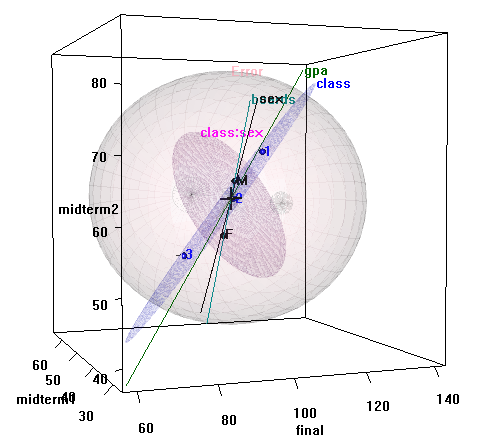
\includegraphics[width=.7\textwidth]{grades-HE3D}
\caption{3D HE plot for SocGrades, model \code{grades.mod3}}
\label{fig:grades-HE3D}
\end{center}
\end{figure}
Interactive
rotation of this plot shows that the effect of \code{class} is only two dimensional,
and of these, one is very small.  The major axis of the \code{class} ellipsoid
is aligned with increasing performance on all three grades, with the expected
ordering of the three social classes.

The representation of these effects in canonical space is particularly useful here.
Again, use \func{candiscList} to compute the canonical decompositions for all terms
in the model, and extract the canonical $R^2$ from the terms in the result.

\begin{Schunk}
\begin{Sinput}
> # calculate canonical results for all terms
> grades.can <- candiscList(grades.mod3)
> # extract canonical R^2s
> unlist(lapply(grades.can, function(x) x$canrsq))
\end{Sinput}
\begin{Soutput}
    class1     class2        sex        gpa     boards class:sex1 class:sex2 
  0.613620   0.024186   0.365269   0.589145   0.472268   0.310461   0.132931 
\end{Soutput}
\end{Schunk}

We use \func{heplot} on the \code{"candiscList"} object to show
the effects of \code{class} in canonical space, giving \figref{fig:grades-can-class}.
\begin{Schunk}
\begin{Sinput}
> # plot class effect in canonical space
>  op <- par(xpd=TRUE)
>  heplot(grades.can, term="class", scale=4, fill=TRUE, var.col="black", var.lwd=2)
>  par(op)
\end{Sinput}
\end{Schunk}
\begin{figure}[htb]
\begin{center}
	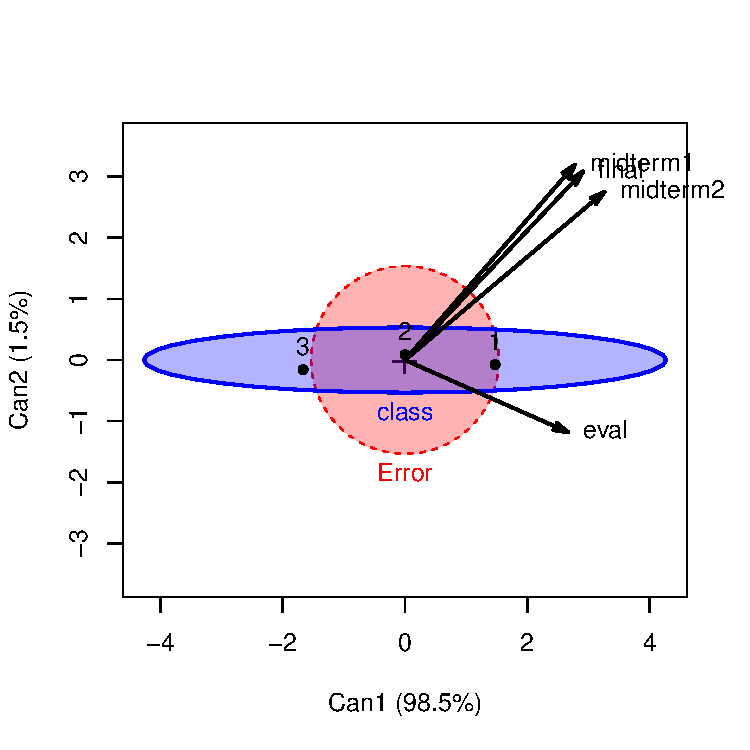
\includegraphics[width=.7\textwidth]{fig/plot-grades-can-class}
\caption{Canonical HE plot for \code{class} effect in  \code{grades.mod3}}
\label{fig:grades-can-class}
\end{center}
\end{figure}

It can be seen in \figref{fig:grades-can-class} that nearly all variation
in exam performance due to class is aligned with the first canonical dimension.
The three tests and course evaluation all have similar weights on this dimension,
but the course evaluation differs from the rest along a second, very small
dimension.

1D plots of the canonical scores for other effects in the model are also of
interest, and provide simple interpretations of these effects on the response
variables.  The statements below produce the plots shown in \figref{fig:grades-can1}.  
\begin{Schunk}
\begin{Sinput}
> plot(grades.can, term="sex")
> plot(grades.can, term="gpa")
\end{Sinput}
\end{Schunk}
\begin{figure}[htb!]
\begin{center}
	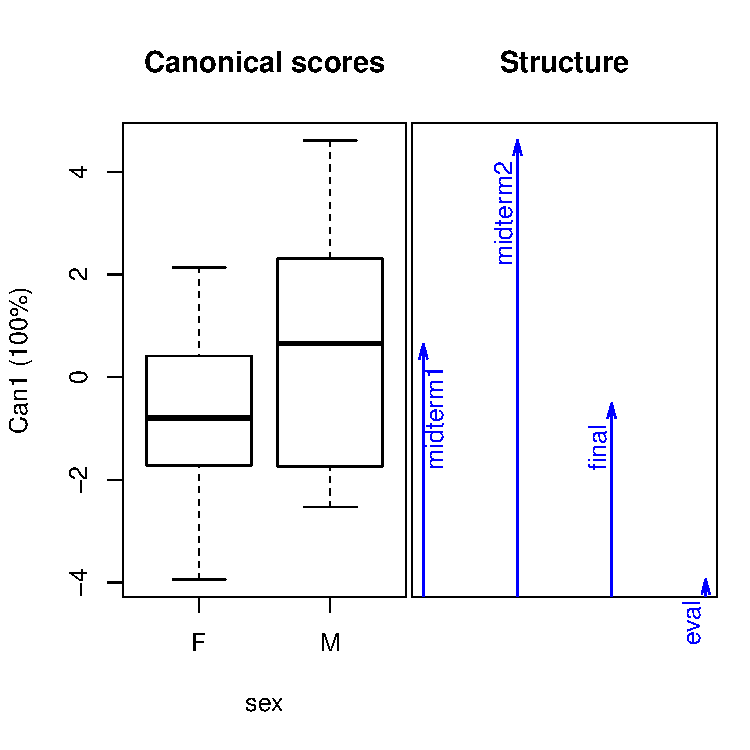
\includegraphics[width=.48\textwidth]{fig/plot-grades-can-sex}
	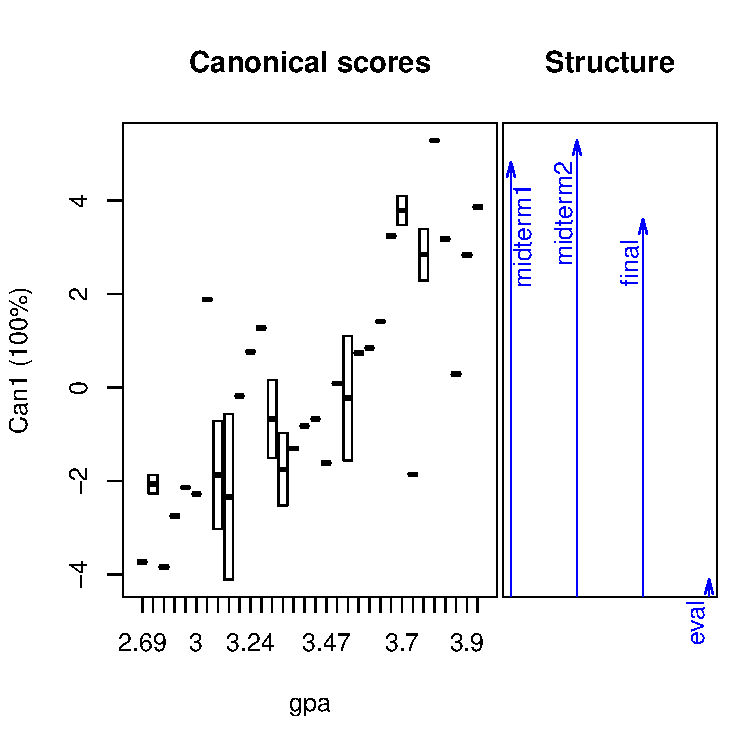
\includegraphics[width=.48\textwidth]{fig/plot-grades-can-gpa}
\caption{1D Canonical discriminant plots for \code{sex} and \code{gpa}.
	Higher canonical scores reflect better course performance.}
\label{fig:grades-can1}
\end{center}
\end{figure}
It is readily seen that males perform better overall, but the effect of
\code{sex} is strongest for the \code{midterm2}.
As well, increasing course performance on tests is strongly associated with
\code{gpa}.  



%\bibliography{graphics}
\bibliography{HE-examples}

\end{document}
